\documentclass[article,A4,12pt]{llncs}
\usepackage[T1]{fontenc}
\usepackage{amsmath}
\usepackage{amssymb}
\usepackage{amsfonts}
\usepackage{mathrsfs, bm}

\usepackage{graphicx}
\usepackage{tabularx}
\usepackage{subfig}
\usepackage{epsf,times}
\usepackage{color}
\usepackage{wrapfig}
\usepackage{cases}
\usepackage{multicol}

\usepackage[T1]{fontenc}
%\newcommand{\tmname}[1]{\textsc{#1}}
%\newcommand{\tmop}[1]{\ensuremath{\operatorname{#1}}}
%\newcommand{\tmsamp}[1]{\textsf{#1}}
%\newcommand{\tmtextsc}[1]{{\scshape{#1}}}
%\newcommand{\tmtextsl}[1]{{\slshape{#1}}}
%\newcommand{\tmtexttt}[1]{{\ttfamily{#1}}}

\leftmargin=0.0cm
\oddsidemargin=0.5cm
\evensidemargin=0.5cm
\topmargin=0cm
\textwidth=16.0cm
%\textheight=21.5cm
\textheight=20.0cm
\pagestyle{plain}
\setlength{\columnsep}{20pt}

\def\m{\mathbf{m}}
\def\H{\mathbf{H}}
\def\E{\mathbf{E}}
\newcommand{\vepsi}{{\varepsilon}}
\def\hnorm#1#2{\vert\,#1\,\vert_{#2}}
\newcommand{\R}{{\mathbb R}}
\newcommand{\Sph}{{\mathbb S}}
\def\x{\mathbf{x}}
\def\hvec{\overline{\mathbf{h}}}
\def\evec{\overline{\mathbf{e}}}

\newcommand{ \etal}{\mbox{\emph{et al. }}}

\newcommand\vect[1]{\mbf{#1}}
\newcommand{\mbf}[1]{\mbox{\boldmath$#1$}} 
\newcommand{\RC}[1]{#1 $\times$ #1 $\times$ #1}
\def\um{$\mu$m}
\def\C{$^{\circ}\mathrm{C}$}

\newcommand{\Rmnum}[1]{\expandafter\@slowromancap\romannumeral #1@}

% DEFINITION OF CUSTOM FONT SIZE
\newcommand{\customfontA}{\fontsize{50}{55}\selectfont}
\newcommand{\customfontB}{\fontsize{14.4}{20}\selectfont}
\newcommand{\customfontC}{\fontsize{30}{35}\selectfont}

\DeclareMathAlphabet{\mathpzc}{OT1}{pzc}{m}{it}

\def\clovek#1{\noindent\bgroup\vbox{\noindent#1}\egroup\vskip1em}

% TO INPUT BACKGROUND IMAGE
\usepackage{eso-pic}
\newcommand\BackgroundPic{
\put(0,0){
\parbox[b][\paperheight]{\paperwidth}{
\vfill
\centering
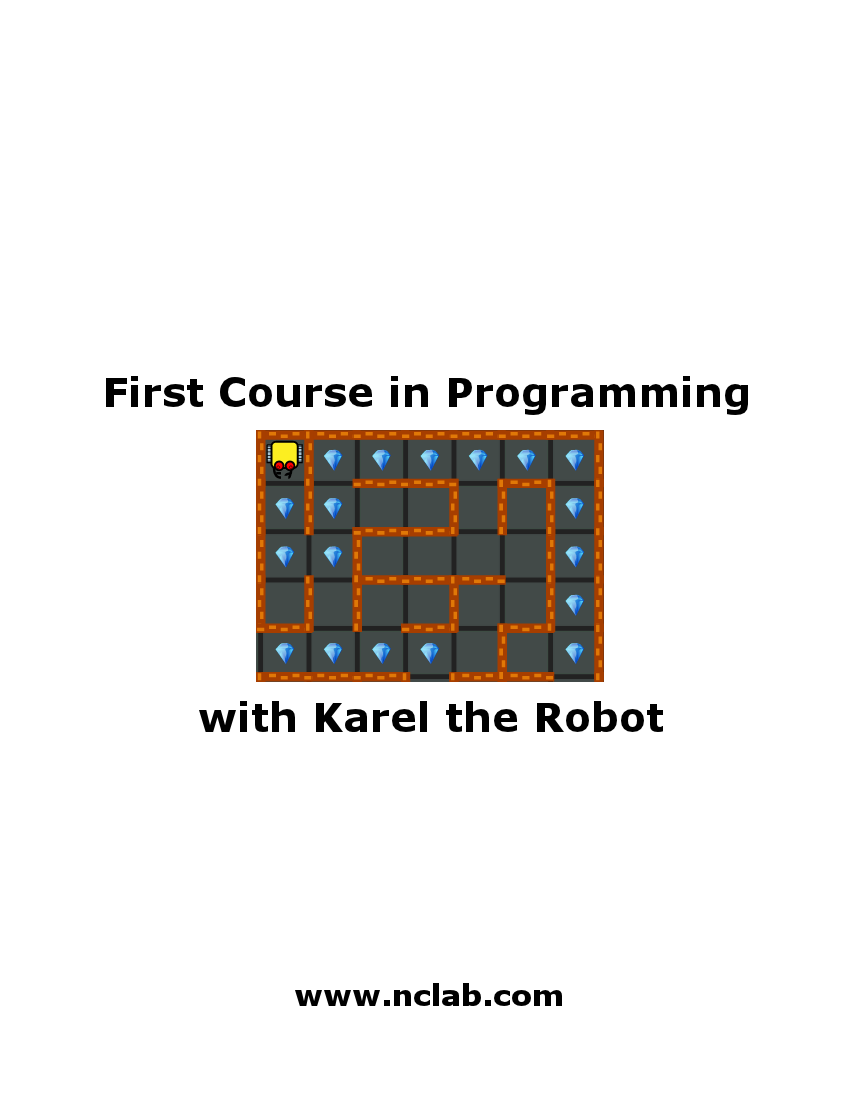
\includegraphics[width=\paperwidth,height=\paperheight]{img/karel-frontpage.png}
%\includegraphics[width=\paperwidth,height=\paperheight]{img/background.jpg}
\vfill
}}}

\begin{document}

% INPUTTING BACKGROUND IMAGE
\AddToShipoutPicture{\BackgroundPic}
\vbox{}
\pagestyle{empty}
\newpage
\textwidth=15.5cm
\ClearShipoutPicture
\newpage

%%%%%%%%%%%%%%%%%%%%%%%%%%%%%%%%%%%%%%%%%%%%%%%%%%%%%%%%%%%%%%%%%%%%%%%%%

\section*{}
\small
\input ../common/aboutnclab.tex

\subsection*{NCLab's Karel vs. the Original Version}
This publication features {\em Karel the Robot}, a programming language 
designed by Richard E. Pattis. Compared to its original version that was
strongly influenced by Pascal, the NCLab version is closer to Python.
There are some other differences as well that make Karel in NCLab easier to use 
for kids -- Karel collects gems instead of beepers, he has a home in the 
maze, and he uses commands that are much easier for kids to understand
and type. For example, {\tt pickbeeper} was replaced with {\tt get}, 
{\tt front-is-clear} was replaced with {\tt wall}, etc. Python 
colons following every command are omitted because using the SHIFT key 
was causing difficulties to some 5 years old programmers. 
Otherwise we have not changed Pattis' original ideas and all functionality 
covered in Pattis' book is available in the Basic Version free of charge. 

\normalsize

\newpage
%{\ }
\setcounter{tocdepth}{2}
\tableofcontents
%\pagestyle{plain}

\newpage

\pagestyle{plain}
\setcounter{page}{1}

%%%%%%%%%%%%%%%%%%%%%%%%%%%%%%%%%%%%%%%%%%%%%%%%%%%%%%%%%%%%%%%%%%%%%%%%%

\section{Introduction}

This course will teach you principles of modern algorithmic design and  
computer programming with the help of an interactive graphical application 
{\em Karel the Robot} in NCLab. Taking this course will make it much easier 
for you to learn Python, C++ and other advanced programming languages. In particular we 
recommend that after Karel you continue with Python, a powerful programming 
language that is used across all science and engineering areas. The textbook
{\em Python Programming for Beginners} is available in PDF via the link 
"Tutorials and Videos" on NCLab home page.

\subsection{Brief history}

Karel the Robot is a famous educational programming language that was introduced by Richard E. 
Pattis in his book "Karel The Robot: A Gentle Introduction to the Art of Programming" in 1981. 
Pattis first used the language in his courses at Stanford University, and now it is used at 
countless schools in the world to introduce students to algorithmic design and computer programming. 
The language is named after Karel \v{C}apek, a Czech writer who invented the word "robot" in his 1921 
science fiction play R.U.R. (Rossum's Universal Robots).

\subsection{Who is Karel?}

Karel is a little robot that lives in a maze, and the maze contains gems that he loves to collect!
He was created with only five simple commands in his memory:
\begin{itemize}
\item {\color{green} \tt go} ... make one step forward.
\item {\color{green} \tt get} ... pick up a gem from the ground. 
\item {\color{green} \tt left} ... turn to the left.
\item {\color{green} \tt right} ... turn to the right. 
\item {\color{green} \tt put} ... put a gem on the ground. 
\end{itemize}
He also has five built-in sensors that allow him to check his immediate surroundings:
\begin{itemize}
\item {\color{green} \tt wall} ... true if he would crash into a wall by making one more step, false otherwise. 
\item {\color{green} \tt gem} ... true if he stands on a gem, false otherwise.
\item {\color{green} \tt north} ... true if he is facing North, false otherwise.
\item {\color{green} \tt home} ... true if he is at home, false otherwise.
\item {\color{green} \tt empty} ... true if his bag with gems is empty, false otherwise. 
\end{itemize}
During this course you will help Karel solve many exciting tasks starting with very simple ones and 
gradually progressing to more challenging. In this way Karel becomes a great robot, and you 
will become a great programmer!

\subsection{Tell me {\em one reason} why I should take this course}

Computer programming skills are highly valued nowadays, and they will be even more 
valued in the future. In this course you will learn to design great algorithms -- an ability that 
is completely language-independent. In other 
words, you can learn the same with a technically complicated conventional 
programming language, battling technical problems most of the time,
or you can learn it with Karel the easy way.
Despite its playful appearance, Karel is {\em not a toy language}. It contains all elements 
of modern procedural programming. The complexity of algorithms 
that you will encounter in this course ranges from {\em extremely simple} 
to {\em extremely tough}.

\subsection{How does Karel differ from conventional programming languages?}

The biggest difference between Karel and conventional procedural
programming languages is that it {\em does not contain any mathematics}.
Believe it or not -- Karel does not know numbers! In this course, you 
will solve many exercises whose objective is to teach you how to 
design great algorithms, and math is not needed for that. 
Thanks to the beautiful simplicity of Karel's language, the resulting 
computer codes are crystal clear.
 
After finishing this tutorial, you will be able to transition instantly to
Python, a powerful modern programming language. And then, you will be only 
learning language-specific details, because the most important skill in computer programming -- designing great algorithms -- you will already have.
 
\section{Explore NCLab}

Before beginning this course, we invite you to create an account in 
NCLab, log in, and take a while to explore the many activities 
that NCLab offers. A great companion reading is {\em Intro to NCLab - Part I 
(Meet the Cloud)} that is available in PDF via the link "Tutorials and Videos"
on NCLab home page {\tt http://nclab.com}.\\

\section{Meet Karel}

Karel can be launched in several different ways. The simplest one is to click on the icon 
"Programming" and select "Karel" in the menu. This will launch the application 
and load a randomly selected maze, as shown in Fig. \ref{fig:init}.

\newpage

\begin{figure}[!ht]
\begin{center}
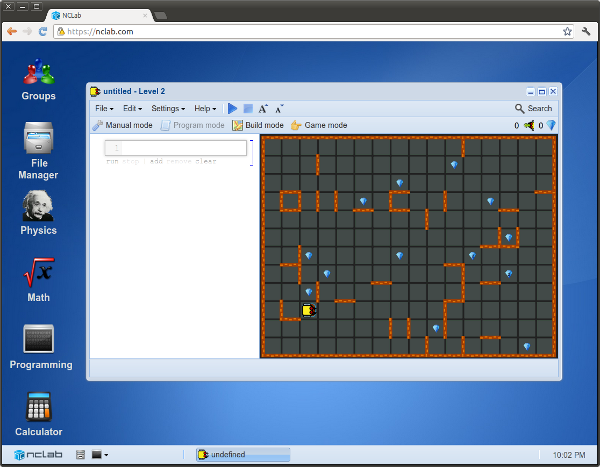
\includegraphics[width=0.9\textwidth]{img/init.png}
\end{center}
%\vspace{-2mm}
\caption{Launching Karel via the Programming icon.}
\label{fig:init}
\end{figure}
\noindent
Karel will be launched in {\em Programming mode} which is the most-frequently 
used one. You can easily switch to the {\em Manual mode}, {\em Builder},
and {\em Game mode} in the menu. Game mode is available in Full Version only. 
These modes will be discussed in more detail later.

\subsection{Cloning Karel projects} \label{cloning}

All programs and games that we will work with are
available for you to clone. To do this, 
click on the File Manager icon. In the File Manager's menu go to 
"Project" and then click on "Clone". This will launch a new window 
with Displayed Projects as shown in Fig. \ref{fig:cloning}.

\newpage

\begin{figure}[!ht]
\begin{center}
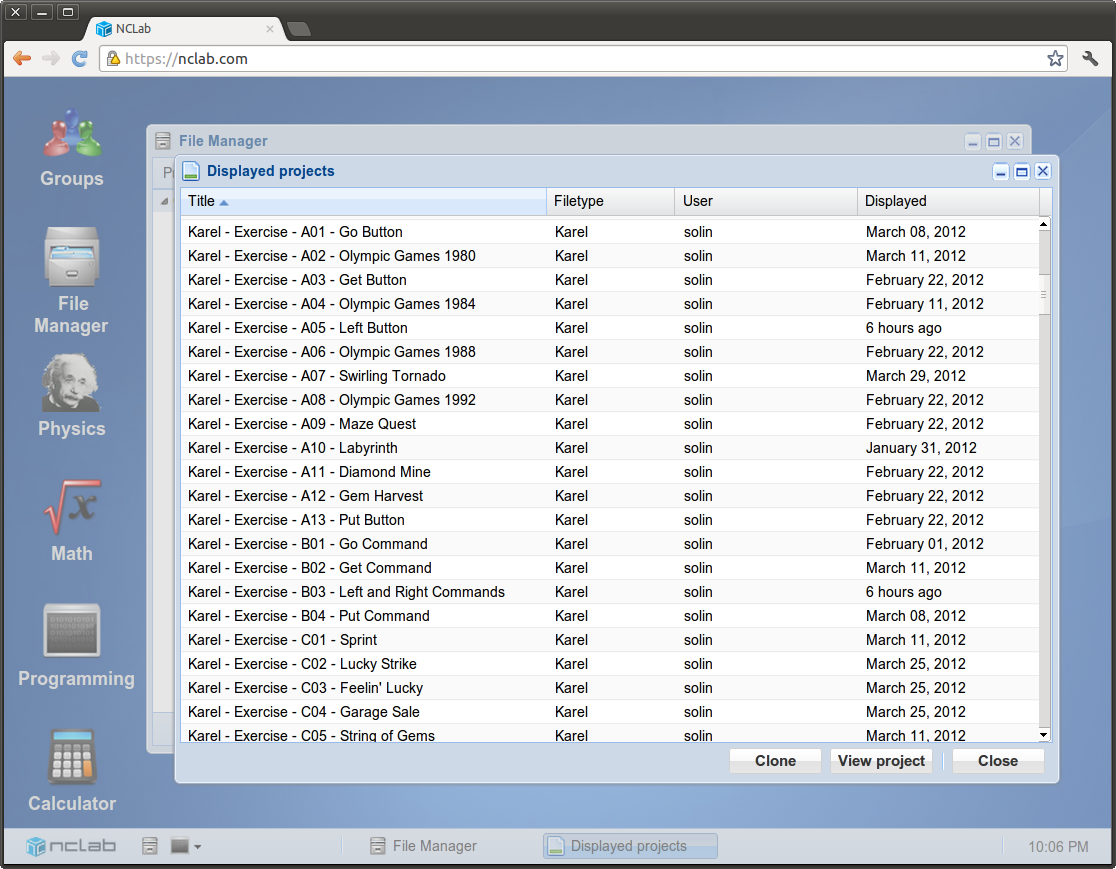
\includegraphics[width=0.9\textwidth]{img/cloning.png}
\end{center}
%\vspace{-2mm}
\caption{File Manager's "Project" menu allows you to clone many Karel projects.}
\label{fig:cloning}
\end{figure}
\noindent
All projects whose names start with "Karel - Exercise" are of particular interest 
for this tutorial. Their solutions have names starting with "Karel - Solution". 
Any of them can be cloned into your account via clicking on the project name in the window, 
and pressing the button "Clone".

In the File Manager's right-hand side panel, you will see the list of all 
projects that you cloned. Click on any of them to launch it. You are free to 
use the cloned projects as they are, or modify them in any way you like. Your 
modifications will not affect the original. And, you can 
always synchronize your version with the original, via 
a right-click on the project in the File Manager and selecting "Synchronize".
Beware though -- synchronizing with the original will erase any changes that 
you made to the project.

\subsection{Basic and Full Versions}

If you are using NCLab in Basic Version, some restrictions apply (this does not concern
institution-sponsored users): The number of saved files is limited, private projects are 
not enabled. and Game mode in Karel is not enabled. Basic Version can be upgraded to Full
via the "Upgrade" icon on desktop.

\subsection{Karel modes}

Karel operates in four modes:
\begin{itemize}
\item {\em Manual mode:} The robot is controlled using the mouse and five buttons Go, Get, Left, Right, and Put. 
      Watch out and do not crash!
\item {\em Program mode:} The robot is controlled using written programs (computer code). The Program mode is 
      split into several Levels:
\begin{itemize}
\item Level 1 is a transition layer between the Manual and Programming modes. Programs are written using only 
      five commands {\tt go}, {\tt get}, {\tt left}, {\tt right}, and {\tt put} that exactly correspond to 
      the buttons Go, Get, Left, Right, and Put in Manual mode.
\item Level 2 is where the actual programming begins. On top of the commands from Level 1, programs can contain 
      conditions, loops, and custom commands.
\item Level 3 teaches the user to operate with logical and numerical variables, and with computer memory. Karel  
      also has receives a GPS device. This Level is in preparation.
\item Level 4 teaches the basics of object-oriented programming. This Level is in preparation.
\item Level 5 teaches the basics of parallel programming. This Level is in preparation.
\end{itemize}
\item {\em Build mode:} This mode allows the user to create custom mazes.
\item {\em Game mode:} Makes it possible to create and play games. 
\end{itemize}

\subsection{Review questions}

\begin{enumerate}
\item Name the university where Karel the Robot was created.
\item What is the biggest difference between Karel and conventional procedural programming languages?
\item Where does Karel live and what objects can be found there?
\item List five commands that Karel knows.
\item What sensors does the robot have?
\item Describe how you would clone a displayed Karel project "Karel - Exercise - C01 - Sprint".
\item What are the four modes of the Karel application?
\item What is the difference between Level 1 and Level 2?
\item What is the most important skill in computer programming?
\item What is the programming language that you should learn after Karel?
\end{enumerate}


\section{Part A - Manual Control}

In the first part you will learn how to guide Karel using the mouse.
There are thirteen games for you to solve. Do not skip levels since each one has something new! Each game can 
be cloned as described in Paragraph \ref{cloning}.. 
Kids as little as 3 years old are playing the games in manual mode, so for you it will be a piece 
of cake. Good luck!

\newpage

\subsection{A01 - Go Button}

{\em Karel is returning from a long walk and his batteries are running out. 
Use the buttons on the left to get him home quickly! }

\begin{figure}[!ht]
\begin{center}
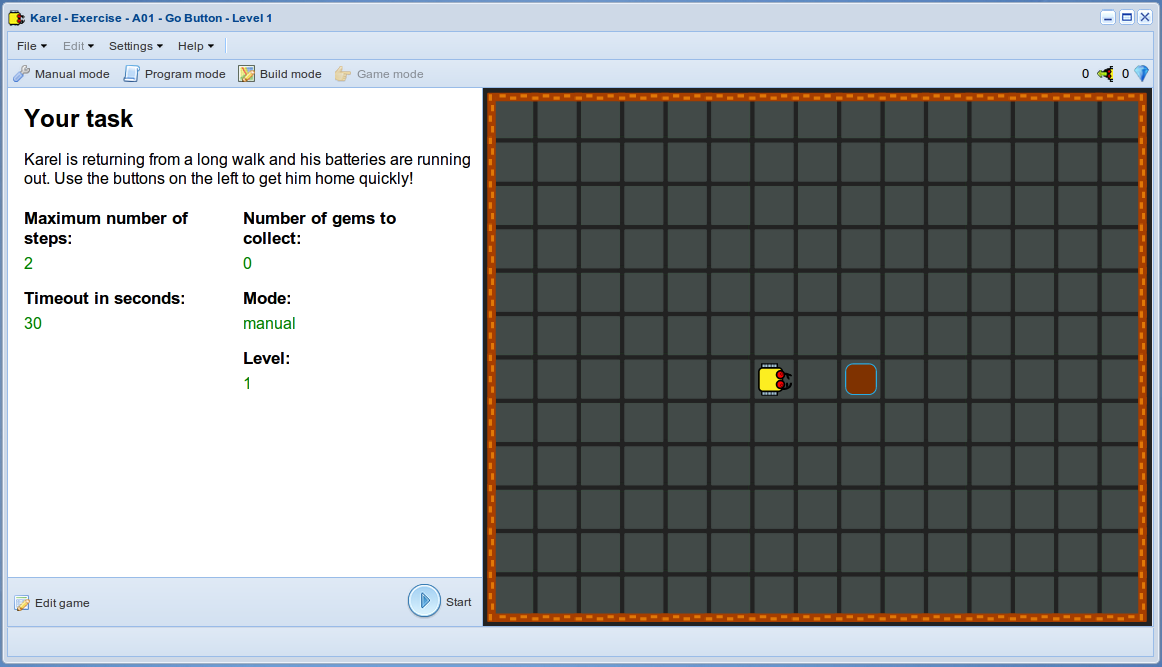
\includegraphics[width=0.7\textwidth]{img/a01.png}
\end{center}
\vspace{-4mm}
\caption{In the first game you need to help the robot get home.}
\label{fig:a01}
\end{figure}
\noindent
Pressing Start will start 
the game, and at this time also the buttons Go, Get, Left, Right, and Put appear, 
as shown in Fig. \ref{fig:a01b}.

\begin{figure}[!ht]
\begin{center}
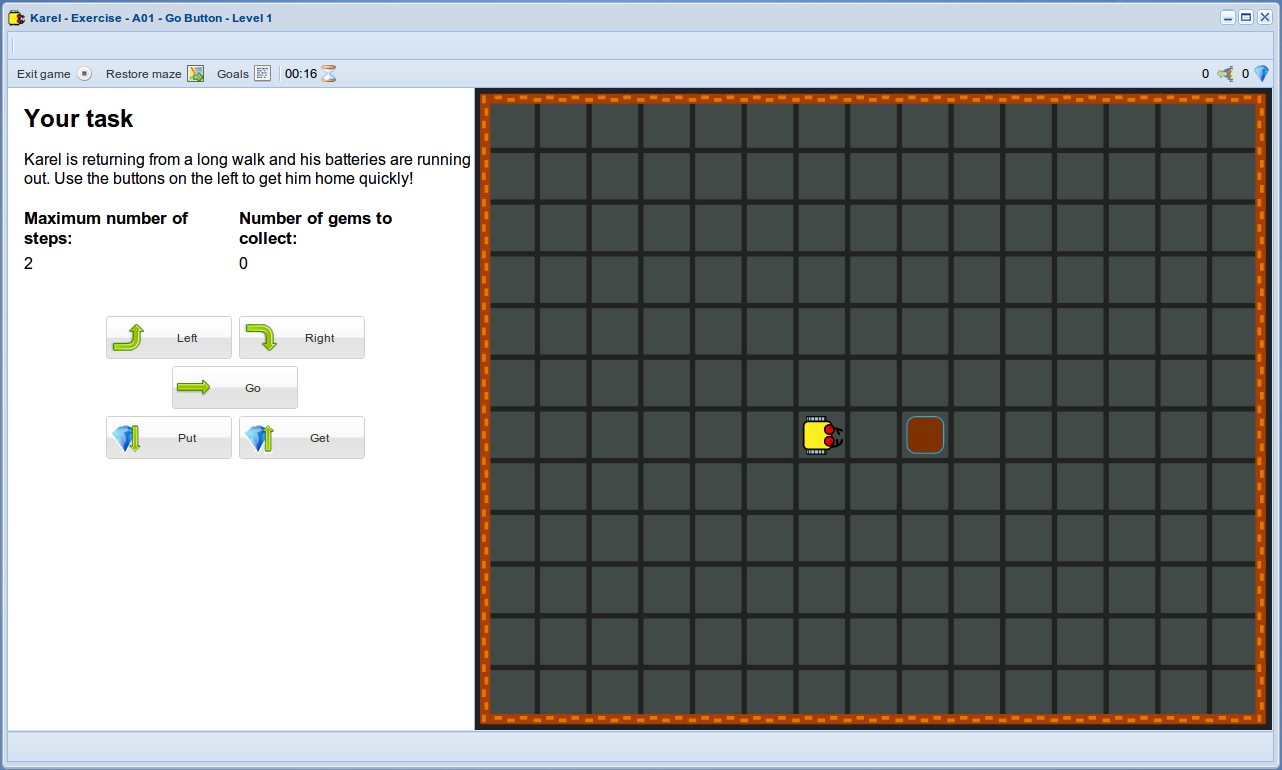
\includegraphics[width=0.7\textwidth]{img/a01b.png}
\end{center}
\vspace{-4mm}
\caption{Karel can be guided manually, using five buttons located in the left panel.}
\label{fig:a01b}
\end{figure}

\newpage

\subsection{A02 - Olympic Games 1980}

{\em Karel is training for Robolympic Games! Your task is to run with 
the robot home as fast as possible. Karel's personal record is four seconds. How fast are you?}

\begin{figure}[!ht]
\begin{center}
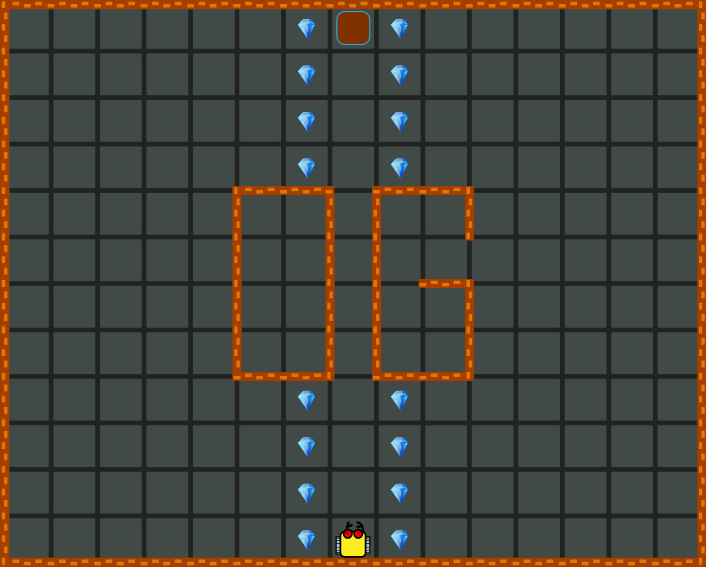
\includegraphics[width=0.7\textwidth]{img/a02.png}
\end{center}
\vspace{-4mm}
\caption{Karel is training for Robolympic Games.}
\label{fig:a02}
\vspace{-4mm}
\end{figure}
\noindent

\subsection{A03 - Get Button}

{\em Today is Karel's lucky day because he is about to find his first gem. 
Use the buttons on the left to help the robot pick up the gem and carry it 
home!}

\begin{figure}[!ht]
\begin{center}
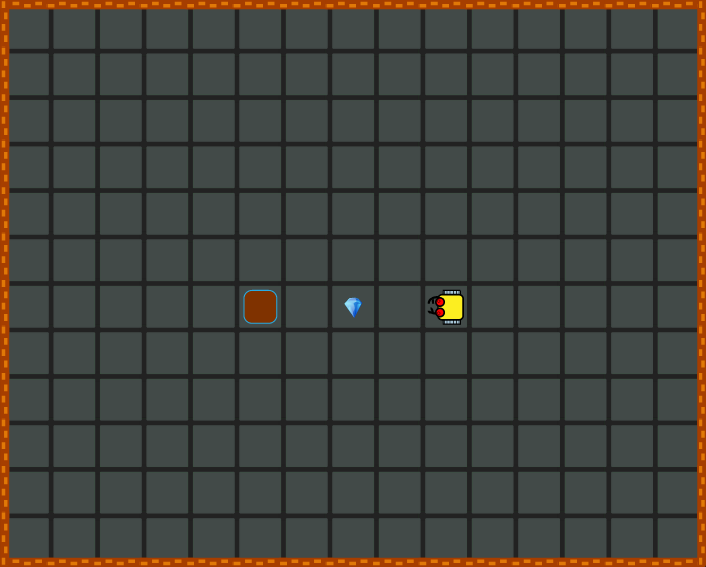
\includegraphics[width=0.7\textwidth]{img/a03.png}
\end{center}
\vspace{-4mm}
\caption{Karel is about to find his first gem.}
\label{fig:a03}
\vspace{-1cm}
\end{figure}
\noindent
\newpage

\subsection{A04 - Olympic Games 1984}

{\em It is Robolympic season again! Run home as fast as you can, 
and collect all three gems on the way! Karel's personal record is 10 seconds.}

\begin{figure}[!ht]
\begin{center}
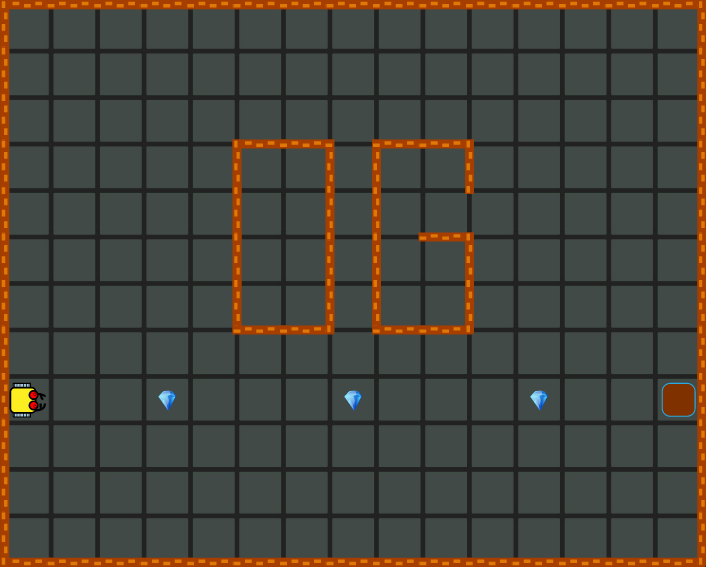
\includegraphics[width=0.7\textwidth]{img/a04.png}
\end{center}
\vspace{-4mm}
\caption{Karel's second Robolympic Games.}
\label{fig:a04}
\end{figure}
\noindent


\subsection{A05 - Left Button}

{\em Help the robot to collect the gem and return home!}

\begin{figure}[!ht]
\begin{center}
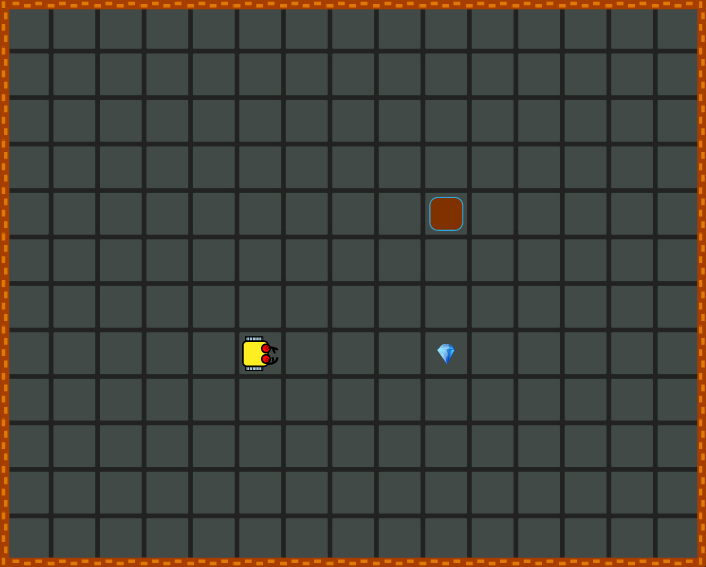
\includegraphics[width=0.7\textwidth]{img/a05.png}
\end{center}
\vspace{-4mm}
\caption{Karel is about to learn how to make a left turn.}
\label{fig:a05}
\vspace{-1cm}
\end{figure}
\noindent
\newpage


\subsection{A06 - Olympic Games 1988 }

{\em Karel is training for his third Robolympic Games. Run with him around the block and home as fast as possible. He needs to collect at least one gem on the way. Karel's personal record is 16 seconds!}

\begin{figure}[!ht]
\begin{center}
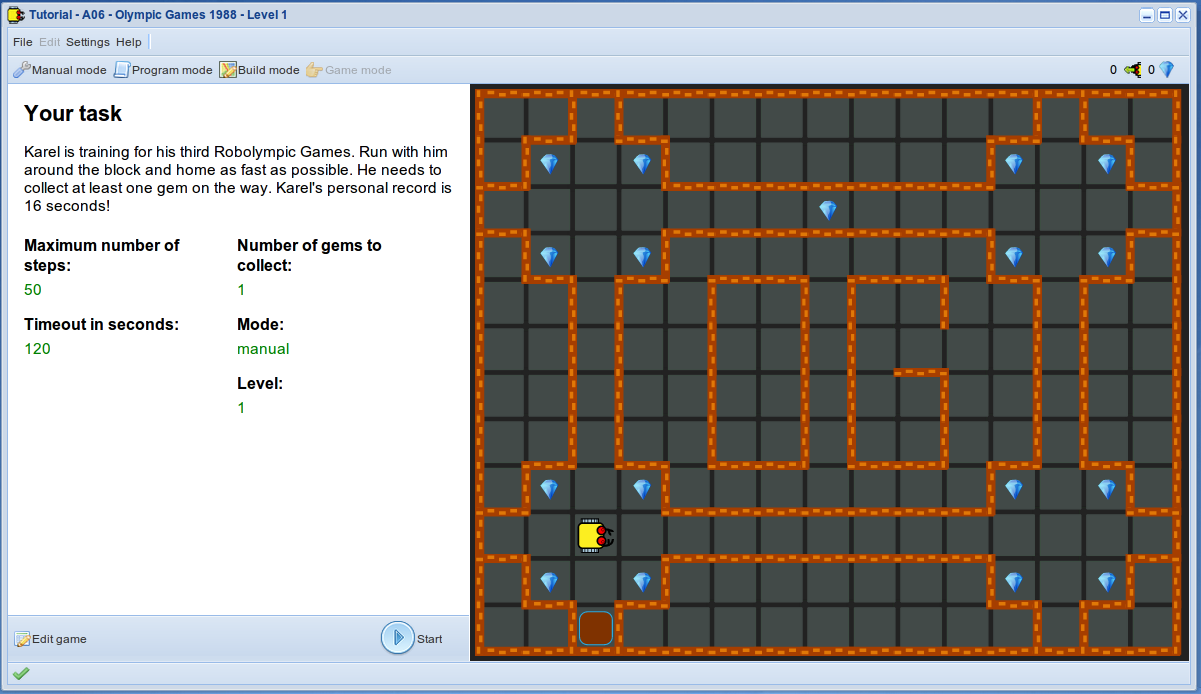
\includegraphics[width=0.7\textwidth]{img/a06.png}
\end{center}
\vspace{-4mm}
\caption{Karel's third Robolympic Games.}
\label{fig:a06}
\end{figure}
\noindent


\subsection{A07 - Right Button}

{\em Pick up the two gems and get Karel home!}

\begin{figure}[!ht]
\begin{center}
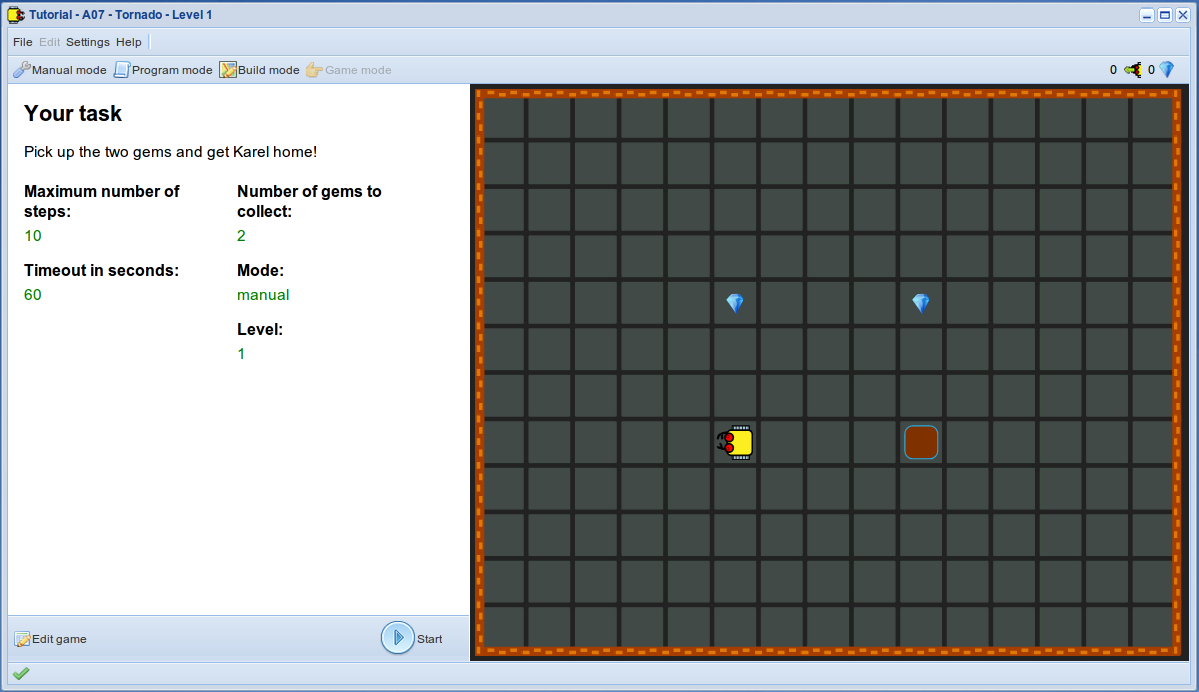
\includegraphics[width=0.7\textwidth]{img/a07.png}
\end{center}
\vspace{-4mm}
\caption{Karel needs to collect two gems and get home.}
\label{fig:a07}
\vspace{-1cm}
\end{figure}
\noindent
\newpage

\subsection{A08 - Olympic Games 1992}

{\em Last season of Karel's Robolympics Games is here! The 
robot needs to run home as fast as possible and bring one gem. 
Be careful not to crash, this is a tricky level! Karel's personal record is 26 seconds.}\\[-7mm]

\begin{figure}[!ht]
\begin{center}
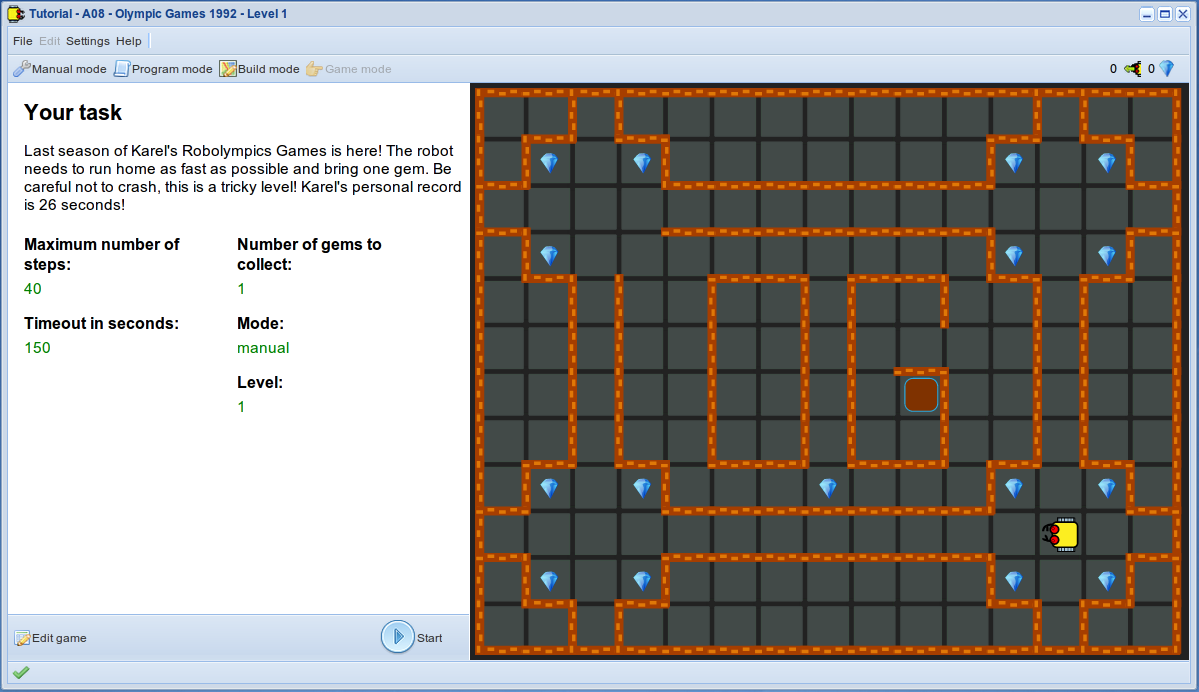
\includegraphics[width=0.7\textwidth]{img/a08.png}
\end{center}
\vspace{-4mm}
\caption{Karel's fourth Robolympic Games.}
\label{fig:a08}
\vspace{-4mm}
\end{figure}
\noindent


\subsection{A09 - Maze Quest}

{\em This time Karel got seriously lost while looking for his favorite gem. 
Help him to collect the gem and find his way home!}\\[-7mm]

\begin{figure}[!ht]
\begin{center}
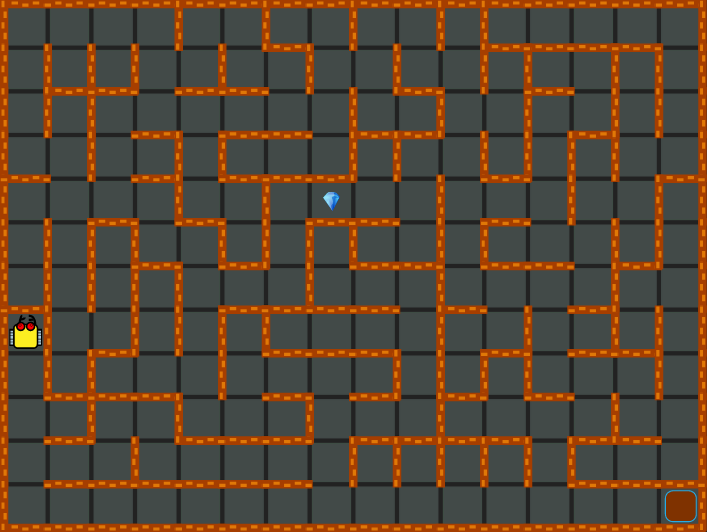
\includegraphics[width=0.7\textwidth]{img/a09.png}
\end{center}
\vspace{-4mm}
\caption{Karel got lost while looking for his favorite gem.}
\label{fig:a09}
\vspace{-4mm}
\end{figure}
\noindent
\newpage

\subsection{A10 - Labyrinth}

{\em This is a true labyrinth and your task is to lead Karel 
home. Remember - think first before going anywhere!}

\begin{figure}[!ht]
\begin{center}
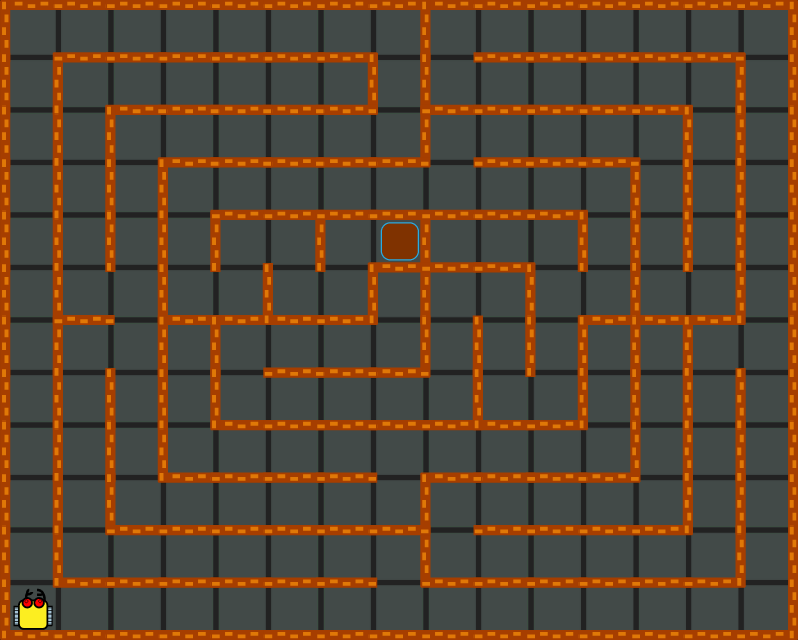
\includegraphics[width=0.7\textwidth]{img/a10.png}
\end{center}
\vspace{-4mm}
\caption{Karel needs to find his way home in a labyrinth.}
\label{fig:a10}
\vspace{-4mm}
\end{figure}
\noindent


\subsection{A11 - Diamond Mine}

{\em Karel discovered an abandoned diamond mine. Use the buttons
on the left to collect all gems and get back home in time!}

\begin{figure}[!ht]
\begin{center}
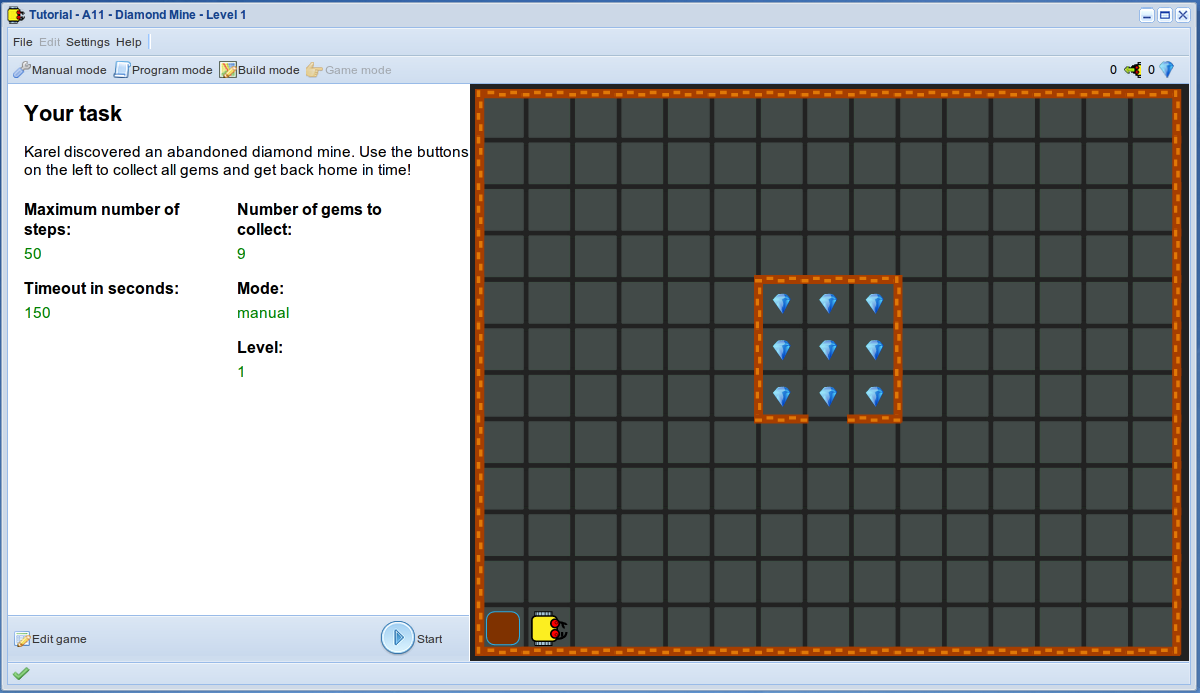
\includegraphics[width=0.7\textwidth]{img/a11.png}
\end{center}
\vspace{-4mm}
\caption{Karel found an abandoned diamond mine.}
\label{fig:a11}
\vspace{-4mm}
\end{figure}
\noindent
\newpage

\subsection{A12 - Gem Harvest}

{\em If gems are piled up, then a number is showing their amount. 
Help Karel collect all gems in this maze and return home!}\\[-7mm]

\begin{figure}[!ht]
\begin{center}
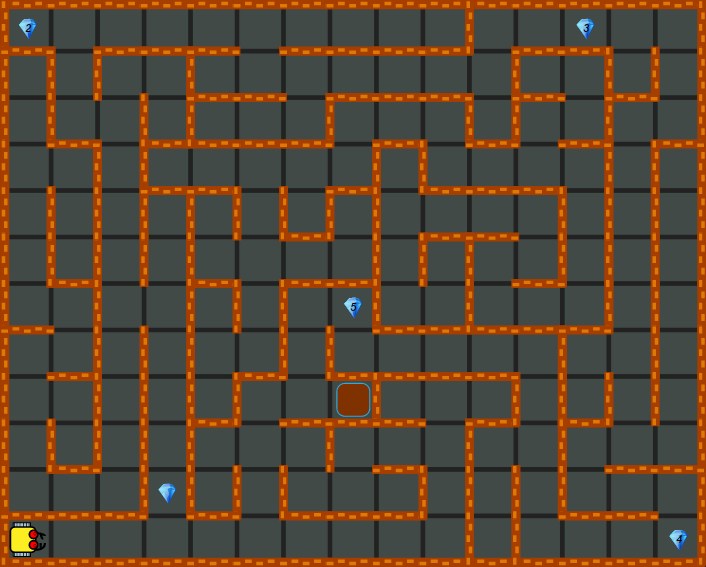
\includegraphics[width=0.7\textwidth]{img/a12.png}
\end{center}
\vspace{-4mm}
\caption{If gems are piled up, then a number is showing their amount.}
\label{fig:a12}
\vspace{-4mm}
\end{figure}
\noindent


\subsection{A13 - Put Button}

{\em Karel has five gems in his bag. Use the buttons on the left to put the gems on the table and 
return home in time!}\\[-7mm]

\begin{figure}[!ht]
\begin{center}
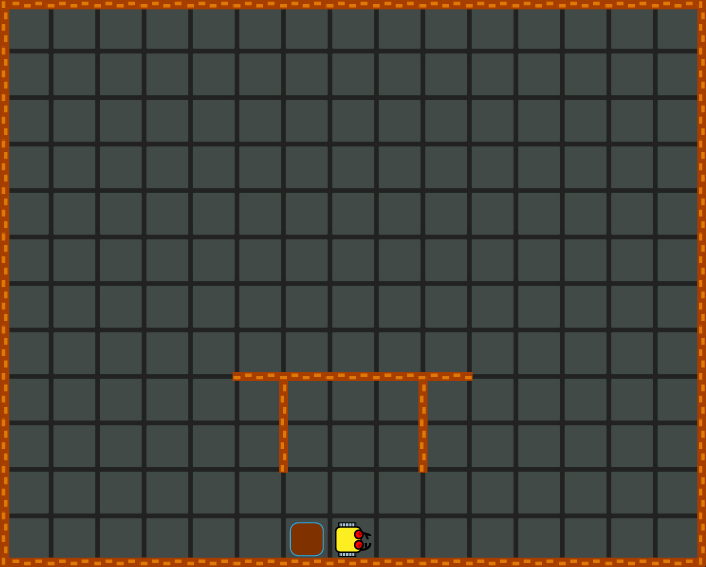
\includegraphics[width=0.7\textwidth]{img/a13.png}
\end{center}
\vspace{-4mm}
\caption{Karel needs to put five gems on the table.}
\label{fig:a13}
\vspace{-4mm}
\end{figure}
\noindent
\newpage

\section{Part B - Bridge to Programming}

Next we will start typing commands {\tt go}, {\tt get}, {\tt left}, {\tt right}, and {\tt put} 
instead of pressing the buttons Go, Get, Left, Right, and Put. You will see that the 
written commands do exactly the same as the buttons!  
There are a couple of simple new rules to remember:
\begin{enumerate} 
\item Commands are typed into an input cell on the left (one will appear after you press Start).
\item Always type one command per line.
\item You can add a new input cell by clicking on "add" (located under each input cell). 
      Having multiple input cells can be useful, for example, to test various versions 
      of your program, or if you want to run parts of your program separately. 
\item Run programs via the blue arrow button in the menu (this will run all 
      cells). Each cell can be run separately by clicking on "run" (located under 
      each input cell). 
\end{enumerate}
You can clone all games in this part into your account via the File Manager's Project
menu, same as you did with the games in Part A, and moreover you can clone their solutions. 
Solution manual in PDF is also provided. 

\subsection{B01 - Go Command}

{\em Write a program that gets Karel home! Remember: Typing "go" is exactly 
the same as pressing the Go button. Always write one command per line.}

\begin{figure}[!ht]
\begin{center}
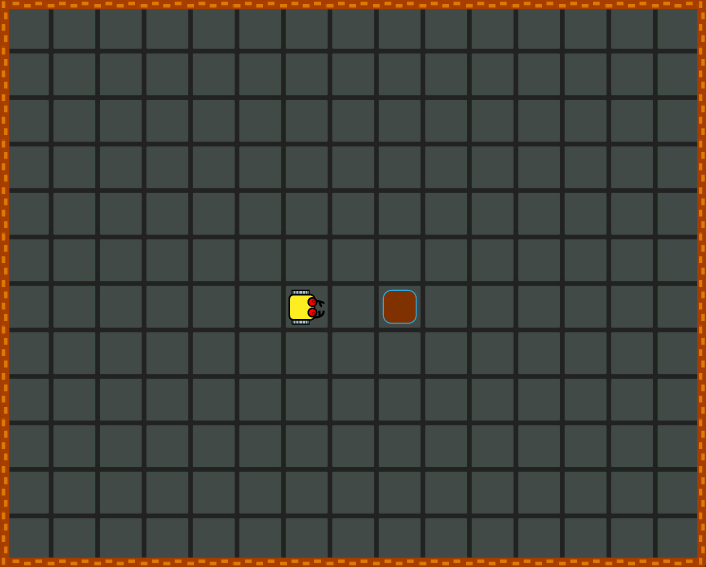
\includegraphics[width=0.7\textwidth]{img/b01.png}
\end{center}
\vspace{-4mm}
\caption{Get Karel home using the {\tt go} command.}
\label{fig:b01}
\vspace{-4mm}
\end{figure}
\noindent

\newpage
\subsection{B02 - Get Command}

{\em Write a program for Karel to collect all gems and get home! 
Remember that typing "get" is the same as pressing the Get button.}\\[-7mm]

\begin{figure}[!ht]
\begin{center}
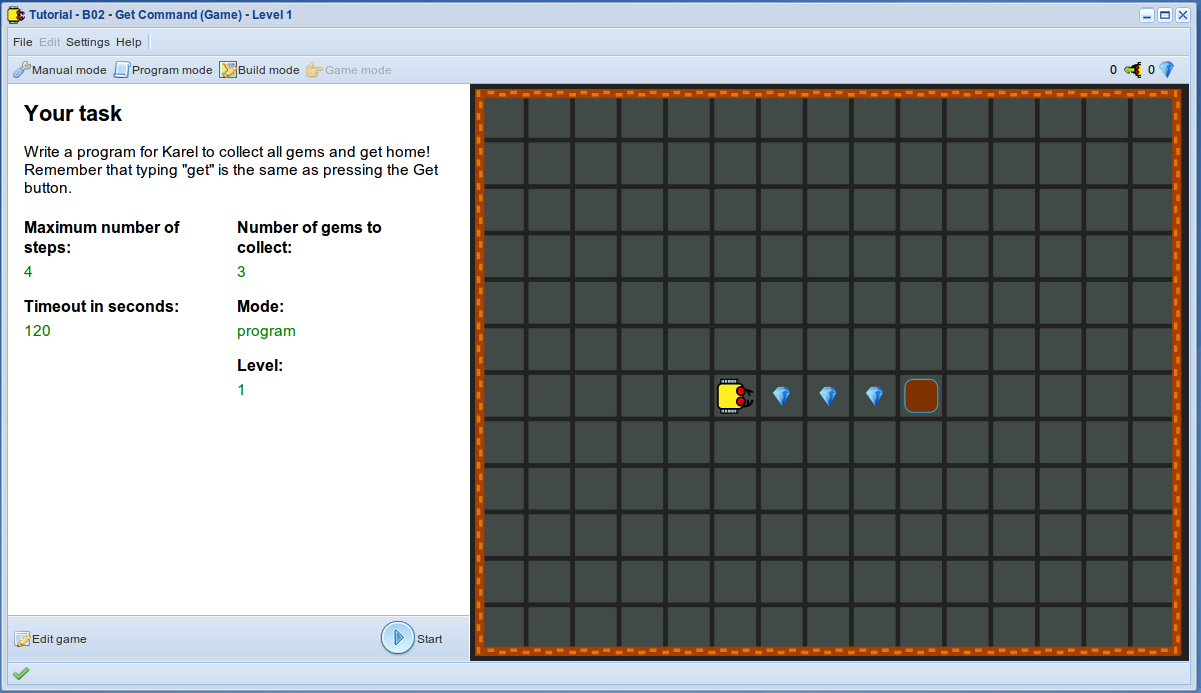
\includegraphics[width=0.7\textwidth]{img/b02.png}
\end{center}
\vspace{-4mm}
\caption{Collecting gems via the {\tt get} command.}
\label{fig:b02}
\vspace{-4mm}
\end{figure}
\noindent

\subsection{B03 - Left and Right Commands}

{\em Write a program for Karel to collect the gem and return 
home! Remember: Typing "left" or "right" is exactly the same as pressing 
the Left or Right button, respectively.}\\[-7mm]

\begin{figure}[!ht]
\begin{center}
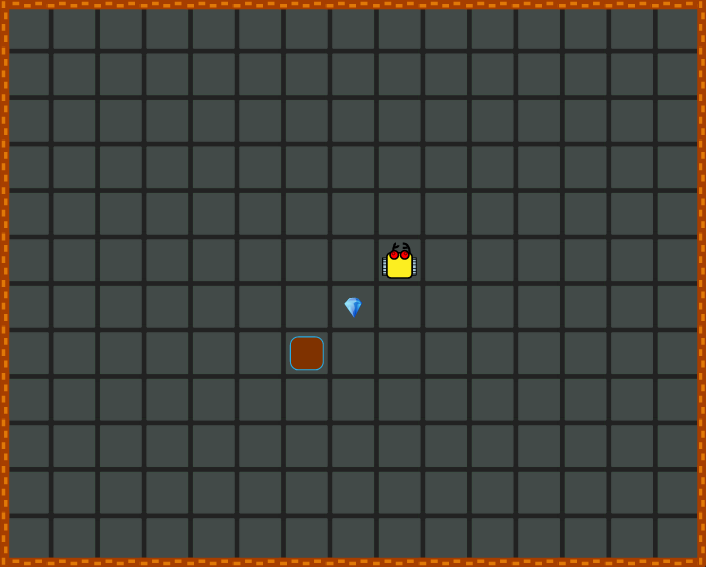
\includegraphics[width=0.7\textwidth]{img/b03.png}
\end{center}
\vspace{-4mm}
\caption{Turning to the left and to the right via the {\tt left} and {\tt right} commands.}
\label{fig:b03}
\vspace{-4mm}
\end{figure}
\noindent
\newpage

\subsection{B04 - Put Command}

{\em Write a program for Karel to pick up the gem, turn around, make 
two steps, put the gem on the ground, and return home! Remember: 
Writing "put" is exactly the same as pressing the Put button.}

\begin{figure}[!ht]
\begin{center}
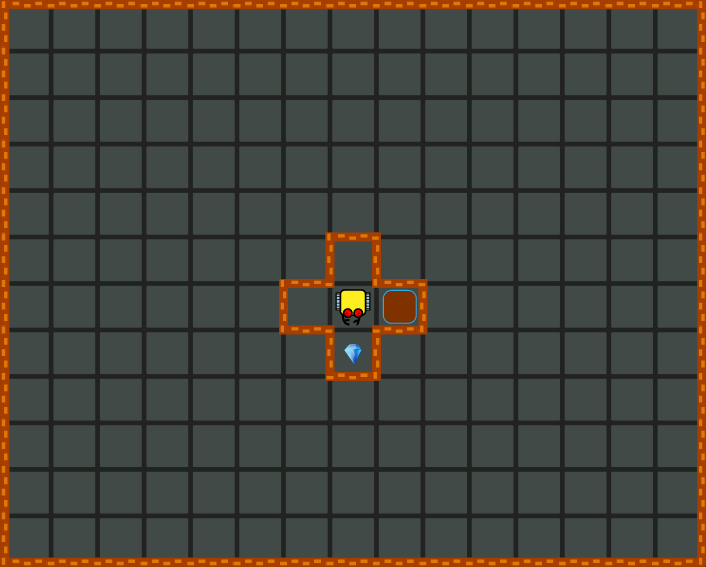
\includegraphics[width=0.7\textwidth]{img/b04.png}
\end{center}
\vspace{-4mm}
\caption{Karel moves a gem from one corner to another using the {\tt put} command.}
\label{fig:b04}
\vspace{-4mm}
\end{figure}
\noindent


\section{Part C - Making It Short and Elegant}

In Part B we learned that Karel accepts written commands as an alternative to 
manual control. He always obeys the commands {\em exactly}. It may happen that 
you plan one thing, tell it to the robot, but the robot does something different.
In that case you need to go back, look at your program, and see where the 
problem is. This is called {\em debugging}. Depending on how careful you 
were while preparing and writing your program, and how complex the program is,
this may take quite a bit of time.

It really helps to be careful and 
think twice before writing a program. You have to go in your mind through 
all the commands that you want the robot to follow. You have to play the program 
in your head, then the robot will do exactly what you want him to do. 

Now we will learn a simple and elegant way to save lots of typing 
by using the {\tt repeat} command. It is very simple. Imagine that you want the
robot to make a 360 degree spin. To do this, he needs to turn four times to the 
left (or to the right, it really does not matter):

\begin{verbatim}
left
left
left
left
\end{verbatim}
But the same can be achieved by telling Karel to {\tt repeat} the {\tt left} command {\tt 4} times:

\begin{verbatim}
repeat 4
  left
\end{verbatim}
Notice that the command {\tt left} is indented by two characters. This is important
because it means that the command {\tt left} is in the {\em body} of the {\tt repeat} 
command. If we want to repeat multiple commands, then all of them need to be indented
like this. For example, to repeat {\tt go} and {\tt left} three times, we type:

\begin{verbatim}
repeat 3
  go
  left
\end{verbatim}
That's it! Enough of studying, now let's go play some games again. 
As before, you can clone all of them via the File Manager's Project menu.

 
\subsection{C01 - Sprint}

{\em Karel's home is ten steps away, so you could type "go" ten times to get him home. However, using the "repeat" command you can do this with only {\bf two lines}! Remember to use an indent of 2 or 4 empty characters on the new line after the {\tt repeat} command.}

\begin{figure}[!ht]
\begin{center}
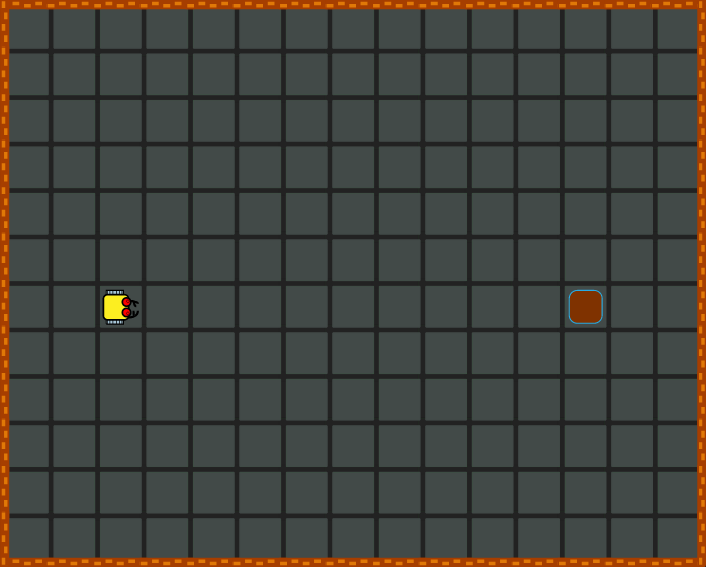
\includegraphics[width=0.7\textwidth]{img/c01.png}
\end{center}
\vspace{-4mm}
\caption{Karel gets home elegantly, using the {\tt repeat} command.}
\label{fig:c01}
\vspace{-4mm}
\end{figure}
\noindent

\newpage

\subsection{C02 - Lucky Strike}

{\em Karel is about to find a pile of 12 gems! Write a program for the robot to collect the gems and get home. Use the {\tt repeat} command for any repeated action. Remember to use an indent of 2 or 4 empty characters on the new line after each {\tt repeat} command. You have to cancel the indentation when the next command to come does no longer belong to the body of the {\tt repeat} command. }

\begin{figure}[!ht]
\begin{center}
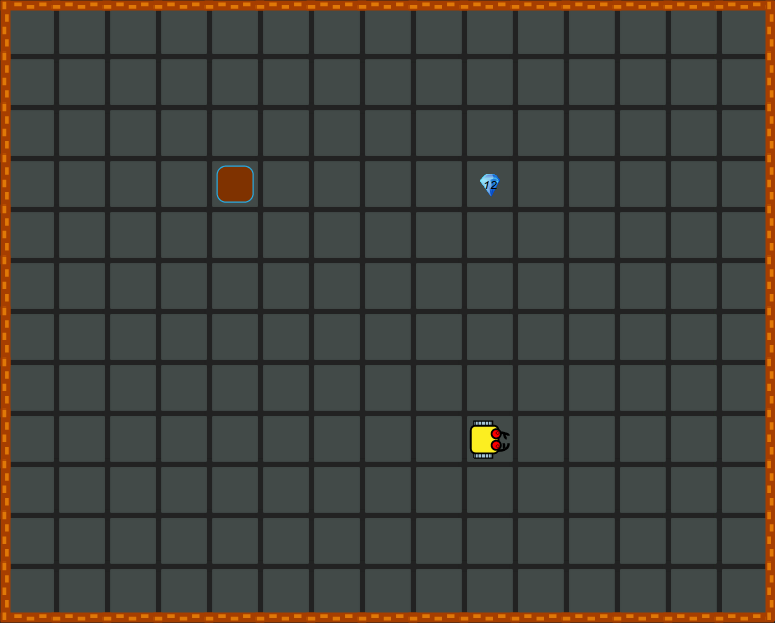
\includegraphics[width=0.7\textwidth]{img/c02.png}
\end{center}
\vspace{-4mm}
\caption{Karel is about to find a pile of 12 gems!}
\label{fig:c02}
\vspace{-4mm}
\end{figure}
\noindent


\subsection{C03 - Feelin' Lucky}

{\em Karel is feeling lucky today. He wants to just step outside his house, 
turn around five times, then pick up one gem somewhere, and get back inside!}

\newpage

\begin{figure}[!ht]
\begin{center}
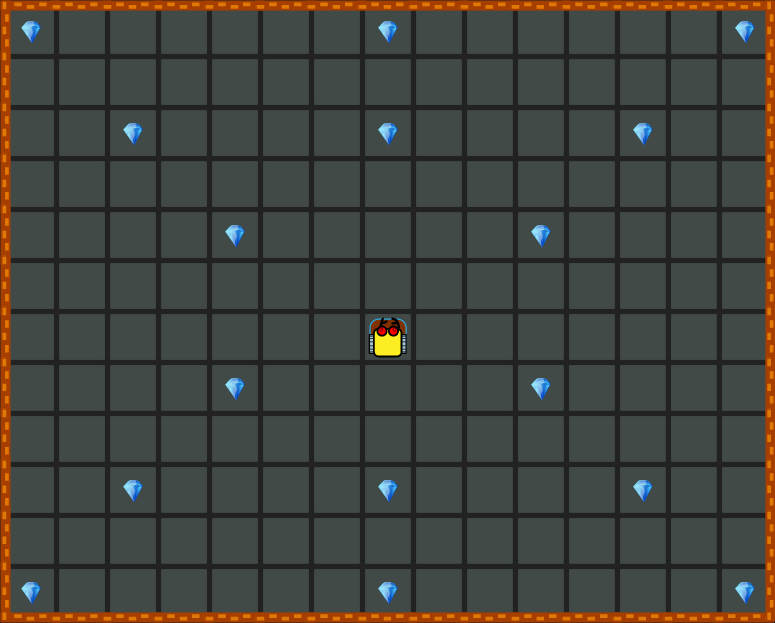
\includegraphics[width=0.7\textwidth]{img/c03.png}
\end{center}
\vspace{-4mm}
\caption{Karel is feeling lucky today.}
\label{fig:c03}
\vspace{-4mm}
\end{figure}
\noindent


\subsection{C04 - Garage Sale}

{\em Karel needs to sell 10 of his oldest gems in order to make space for new ones. 
Write a program for the robot to step out of his garage, put 10 gems on the ground, 
and then turn back and get back inside! Use the {\tt repeat} command for any repeated 
action.}

\begin{figure}[!ht]
\begin{center}
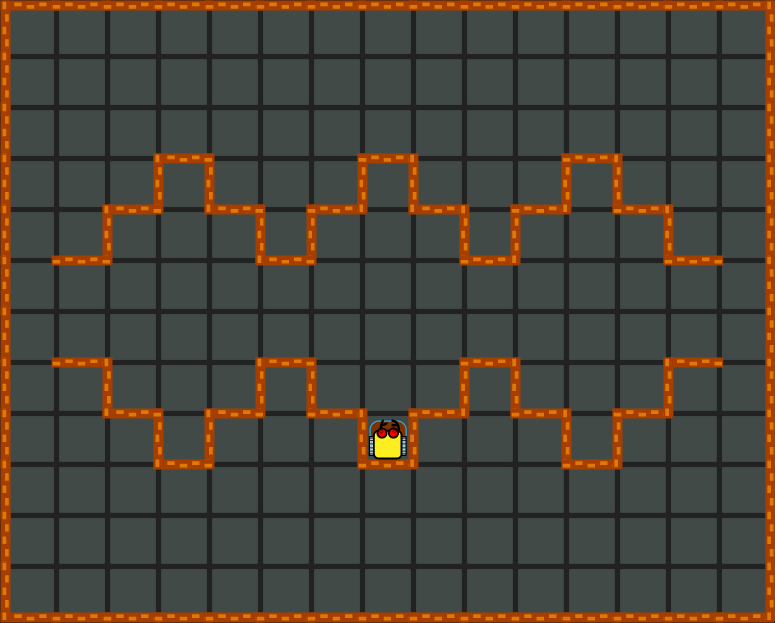
\includegraphics[width=0.7\textwidth]{img/c04.png}
\end{center}
\vspace{-4mm}
\caption{Karel is getting ready for garage sale.}
\label{fig:c04}
\vspace{-4mm}
\end{figure}
\noindent


\newpage


\subsection{C05 - String of Gems}

{\em Write a program for Karel to collect all nine gems and get home! 
Writing one command per line, your program should not have more 
than three lines.}.

\begin{figure}[!ht]
\begin{center}
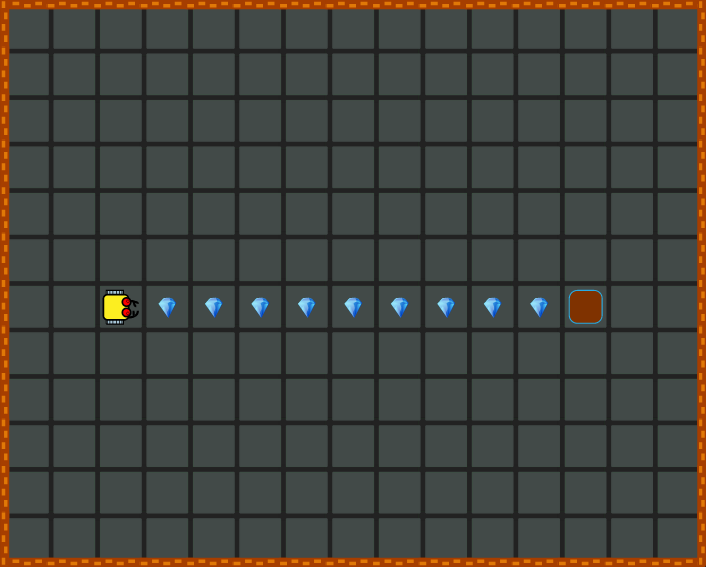
\includegraphics[width=0.7\textwidth]{img/c05.png}
\end{center}
\vspace{-4mm}
\caption{Nine gems are between Karel and his home.}
\label{fig:c05}
\vspace{-4mm}
\end{figure}
\noindent

\section{Part D - Sensors and Conditions}

Karel has five built-in sensors to better navigate in the maze. 
The first one is an infrared sensor that the robot uses to determine 
whether it is safe to move forward, or whether there is a wall ahead.
The usage can be illustrated using a simple program "Careful step" 
where Karel first checks whether there is a wall ahead before
making a step. If there is wall, he turns back: 

\begin{verbatim}
# Program "Careful step".
if wall
  repeat 2
    left
else
  go
\end{verbatim}
Note that the symbol {\tt \#} introduces a comment, meaning that the line 
of code behind it is ignored by the robot.
The {\tt else} branch does not have to be there if it is not needed. Notice the indentation 
of the bodies of the {\tt if} and {\tt else} branches - this is analogous 
to how we indent the body of the {\tt repeat} command.

Besides {\tt wall}, the robot can check the following:
\begin{itemize}
\item {\tt gem} ... is there a gem where he stands?
\item {\tt empty} ... is his bag with gems empty?
\item {\tt north} ... is he facing North?
\item {\tt home} ... is he at home?
\end{itemize}
Karel can also use the reserved word {\tt not} to test the opposites.
For illustration, the previous program can be rewritten as follows, without changing its function:
\begin{verbatim}
# Program "Careful step".
if not wall
  go
else
  repeat 2
    left
\end{verbatim}

\subsection*{Errors}
This is important: If you crash the robot into a wall, if you ask him to collect a gem where there
is none, or if you ask him to put a gem on the ground while 
his bag is empty, {\bf he will throw an error.}. This means that 
he will write a complaint for you, and he will stop executing the program. 


\subsection{D01 - In the Fog}

{\em Several gems lie on the ground between the robot and his home which is 10 steps away. 
He cannot see where they are exactly since his sensor only tells him if a gem is right 
under him.  And besides that, nothing is visible in today's foggy weather anyway. 
Write a program for Karel to collect all gems and get home. With one command per 
line, your program should have at most 4 lines.}


\begin{figure}[!ht]
\begin{center}
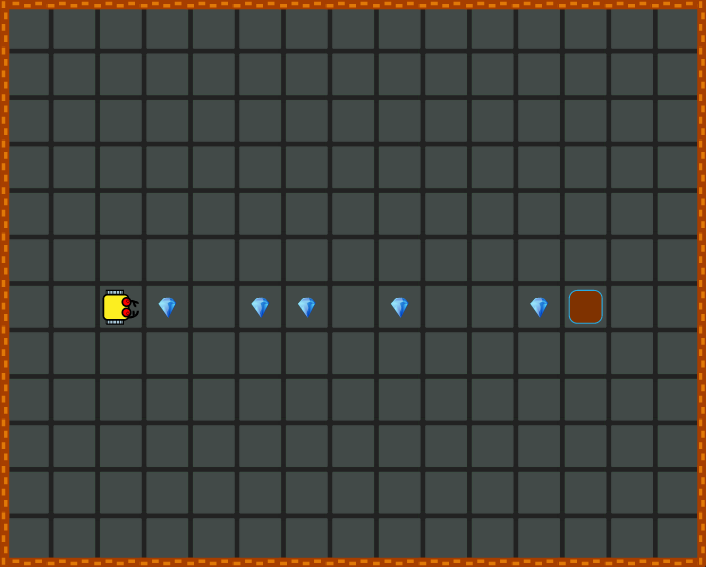
\includegraphics[width=0.7\textwidth]{img/d01.png}
\end{center}
\vspace{-4mm}
\caption{With zero visibility, Karel needs to rely on his sensors.}
\label{fig:d01}
\vspace{-4mm}
\end{figure}
\noindent

\newpage

\subsection{D02 - Stony Meadows}

{\em Karel is walking on a meadows that is covered with irregularly 
scattered stones. Write a program for the robot to get to his home, 
avoiding stones, and collecting all three gems!  }


\begin{figure}[!ht]
\begin{center}
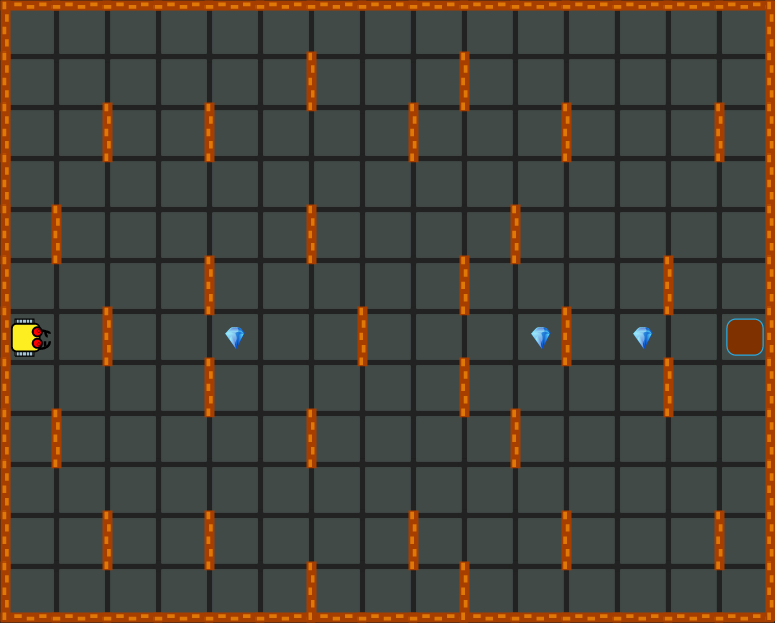
\includegraphics[width=0.7\textwidth]{img/d02.png}
\end{center}
\vspace{-4mm}
\caption{Karel is crossing a stony meadows.}
\label{fig:d02}
\vspace{-4mm}
\end{figure}
\noindent





\subsection{D03 - Filling the Blanks}

{\em Karel stores all his gems in a secret chest in his cellar. 
Currently, some shelves are empty. Write a program for Karel to 
inspect all shelves and put a gem where one is missing! After that, he needs to get 
home as usual. With one 
command per line, your program should have at most 7 lines.}


\begin{figure}[!ht]
\begin{center}
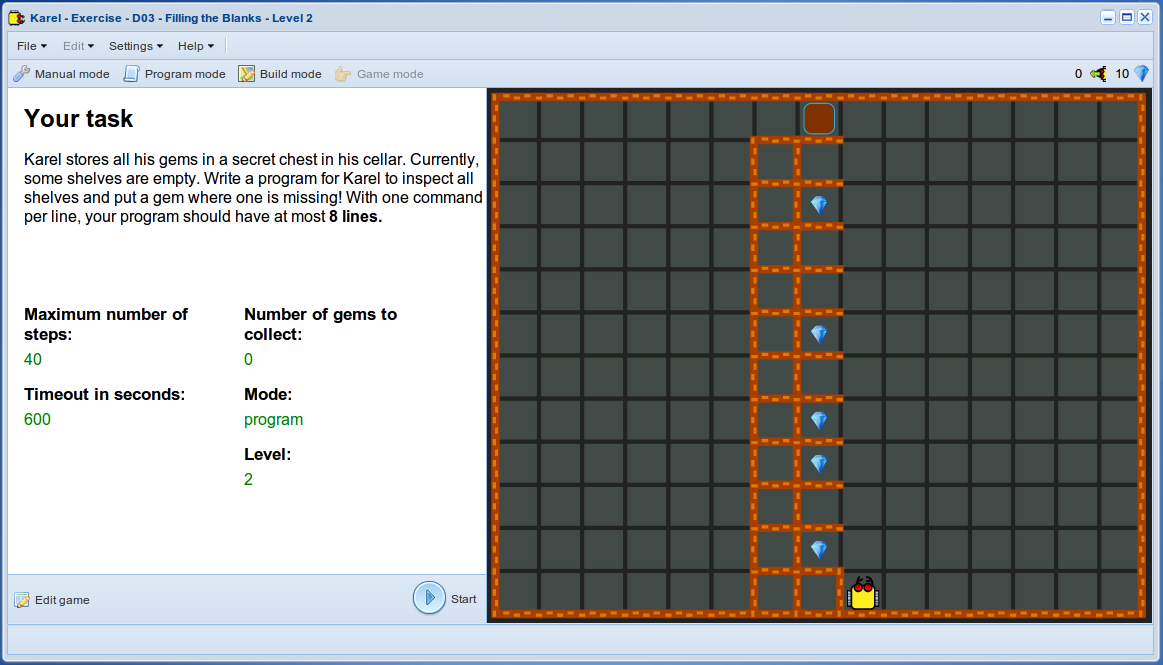
\includegraphics[width=0.7\textwidth]{img/d03.png}
\end{center}
\vspace{-4mm}
\caption{Filling his secret chest with gems.}
\label{fig:d03}
\vspace{-4mm}
\end{figure}
\noindent



\section{Part E - The Smart Loop}

Sometimes Karel needs to repeat something not knowing how many repetitions
there will be. This can be the case, for example, 
when he is asked to walk straight ahead until he reaches the closest wall
(remember that he only can see walls that are right ahead of him; walls 
that are further away he can't see). Such a program would be:

\begin{verbatim}
while not wall
  go
\end{verbatim}
Or, he may be asked to walk until he gets home:

\begin{verbatim}
while not home
  go
\end{verbatim}
Or, he may be asked to empty his bag (he does not know how many gems are in it): 
 
\begin{verbatim}
while not empty
  put
\end{verbatim}
Or, he may be asked to collect all gems from a pile (he does not know 
how many gems there are):

\begin{verbatim}
while gem
  get
\end{verbatim}
Or we may ask him to turn to face North (he does not know which direction he is
facing):

\begin{verbatim}
while not north
  left
\end{verbatim}
At last, Karel is asked to 
turn South, walk straight ahead until he reaches the closest wall, and 
collect all gems that he can find on the way:

\begin{verbatim}
# First turn North.
while not north
  left

# Then turn South.
repeat 2
  left

# Go straight ahead and pick all gems.
while not wall
  if gem
    get
  go

# Pick gem at the wall (if any).
if gem
  get
\end{verbatim}
Notice that we first need to turn the robot to face North -- this is because North 
is the only direction that he can check!

\subsection{E01 - South West}

{\em Karel is lost and he does not even know whether he is facing north, south, east or west! He only knows that his home is in the south-west corner of the maze. Write a program for the robot to get there. Hint: First you need to orient the robot to face north, that's the only direction that he can check with his sensors.}

\newpage

\begin{figure}[!ht]
\begin{center}
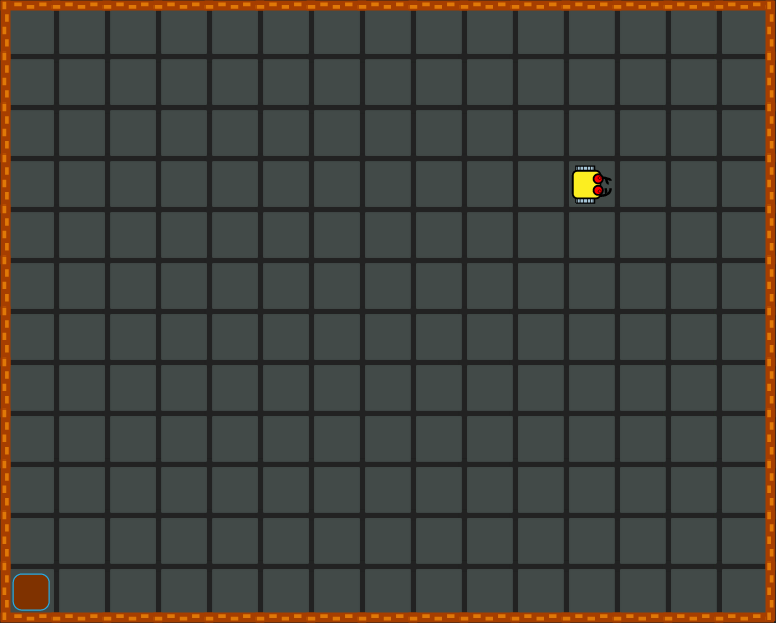
\includegraphics[width=0.7\textwidth]{img/e01.png}
\end{center}
\vspace{-4mm}
\caption{Karel only knows that his home is in the SW corner of the maze.}
\label{fig:e01}
%\vspace{-12mm}
\end{figure}
\noindent


\subsection{E02 - Hide-and-Seek}

{\em Karel's friends are hiding. He knows that he has to go straight 
ahead to find them. When he finds a gem, he has to turn left and keep 
walking. Eventually, he will get to the place where his friends are 
hiding. If he gets home, stop. Write a program for Karel to do this, 
and do not forget to collect all the gems on the way!}\\[-4mm]

\begin{figure}[!ht]
\begin{center}
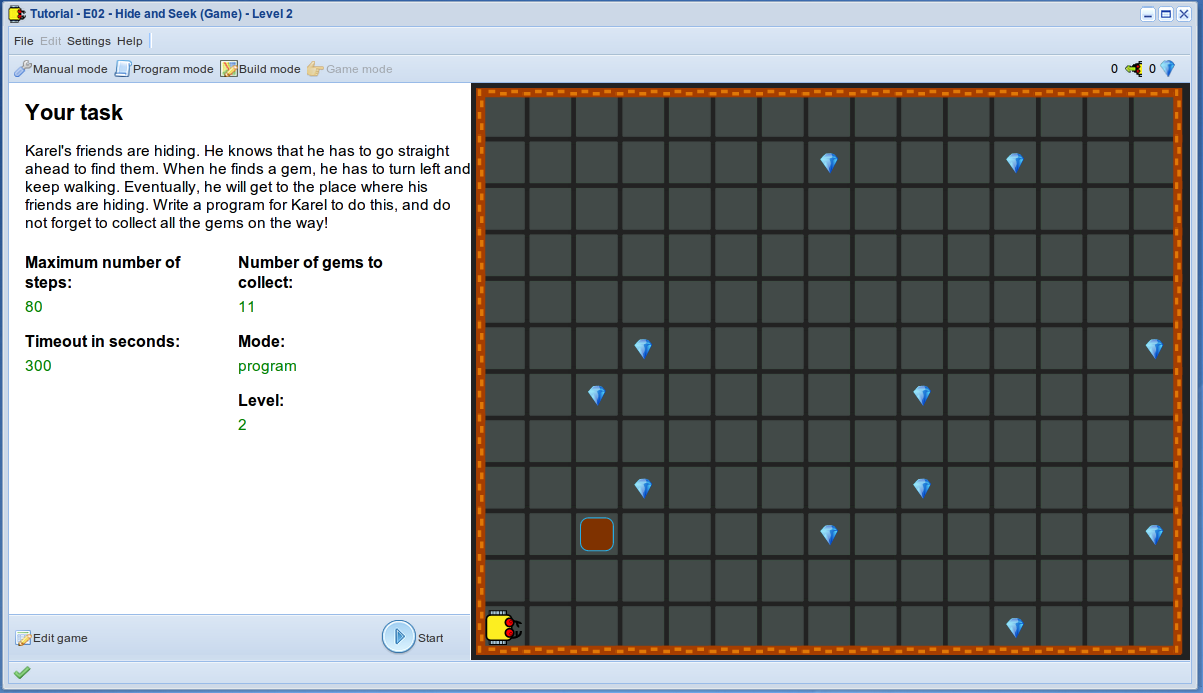
\includegraphics[width=0.7\textwidth]{img/e02.png}
\end{center}
\vspace{-4mm}
\caption{Karel plays hide-and-seek with his friends.}
\label{fig:e02}
\vspace{-10mm}
\end{figure}
\noindent
\newpage

\subsection{E03 - Walk the Line}

{\em Karel stands next to a straight wall and he knows that his home is somewhere on the other side of it. He does not know how long the wall is, nor the exact position of his home. Write a program for the robot to get there!}

\begin{figure}[!ht]
\begin{center}
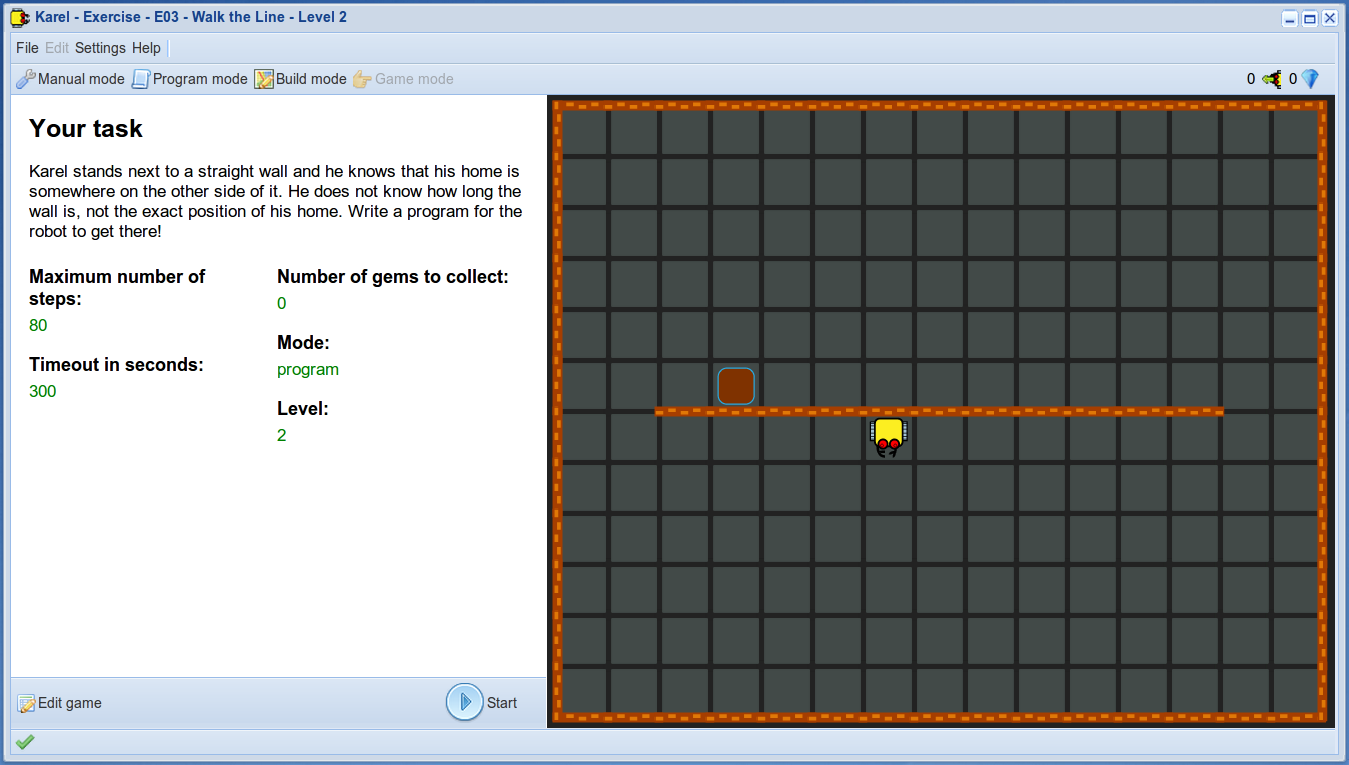
\includegraphics[width=0.7\textwidth]{img/e03.png}
\end{center}
\vspace{-4mm}
\caption{Karel only knows that his home is on the other side of the wall.}
\label{fig:e03}
\vspace{-10mm}
\end{figure}
\noindent

\section{Part F - Defining Custom Commands}

\noindent
{\em Always look for small tasks that can be solved independently of the big ones.
Solve the small tasks first, and you'll see that the big task gets simpler. The 
importance of what we just said cannot be stressed more. Please read these three 
lines once more.}\\

\noindent
The fact that you are reading this line of text proves that you are not 
a perfect programmer yet. Otherwise you would be stuck forever in the 
previous paragraph that is an infinite loop!

\begin{figure}[!ht]
\begin{center}

\includegraphics[width=0.3\textwidth]{img/smiley.png}
\end{center}
\vspace{-1cm}
\end{figure}

\newpage

\subsection*{Defining new commands}
New commands for simpler tasks are defined using the reserved word 
{\tt def}. For example, in a program where the robot needs to turn back
many times, it is a good idea to define a new command {\tt back}
as follows:

\begin{verbatim}
def back
  repeat 2
    left
\end{verbatim}

\subsection*{Revisiting exercise A07}

Let us return to the exercise A07 - Right Button for a moment.
A really bad program to solve this task would be:

{\small
\begin{verbatim}
right
go
go
go
go 
get
right
go
go
go
go 
get
right
go
go
go
go
get
\end{verbatim}
}
\noindent
Can you see how many times the same code is repeated?! In order to fix this, 
we should define new command {\tt foursteps} as
follows:

{\small
\begin{verbatim}
def foursteps
  repeat 4
    go
\end{verbatim}
}
\noindent
With this new command, the above code simplifies to 

{\small
\begin{verbatim}
right
foursteps
get
right
foursteps
get
right
foursteps
get
\end{verbatim}
}
\noindent
There are still repetitions that must be eliminated! So we define a new command 
{\tt walkedge}:

{\small
\begin{verbatim}
def walkedge
  right
  foursteps
  get
\end{verbatim}
}
\noindent
Now with the new commands {\tt foursteps} and
{\tt walkedge}, our program simplifies to:

{\small
\begin{verbatim}
while not home
  walkedge
\end{verbatim}
}
\noindent
It is the task of the first game in this part to implement this program. But before we 
do so, let us mention one very important thing.

\subsection*{Solution procedure revisited (and corrected)}


An experienced programmer would never solve the problem the way we did.
He would first look at the problem, trying to recognize repeating patterns. 
He would find that the task can be fulfilled by repeating one simpler task 
three times. So, without knowing exactly how the smaller task is going to 
be solved, he would write:

{\small
\begin{verbatim}
while not home
  walkedge
\end{verbatim}
}
\noindent
Next he would define the new command {\tt walkedge} as follows:

{\small
\begin{verbatim}
def walkedge
  right
  foursteps
  get
\end{verbatim}
}
\noindent
He would not bother defining the command 
{\tt foursteps} yet, because he knows that this will be 
simple. And as the last step, to make the program work, he would 
define:

{\small
\begin{verbatim}
def foursteps
  repeat 4
    go
\end{verbatim}
}
\noindent
Keep this in mind while solving the following problems!

\newpage

\subsection{F01 - Four Star Hotel}

{\em Before getting home, Karel has to collect all four stars of gems!}


\begin{figure}[!ht]
\begin{center}
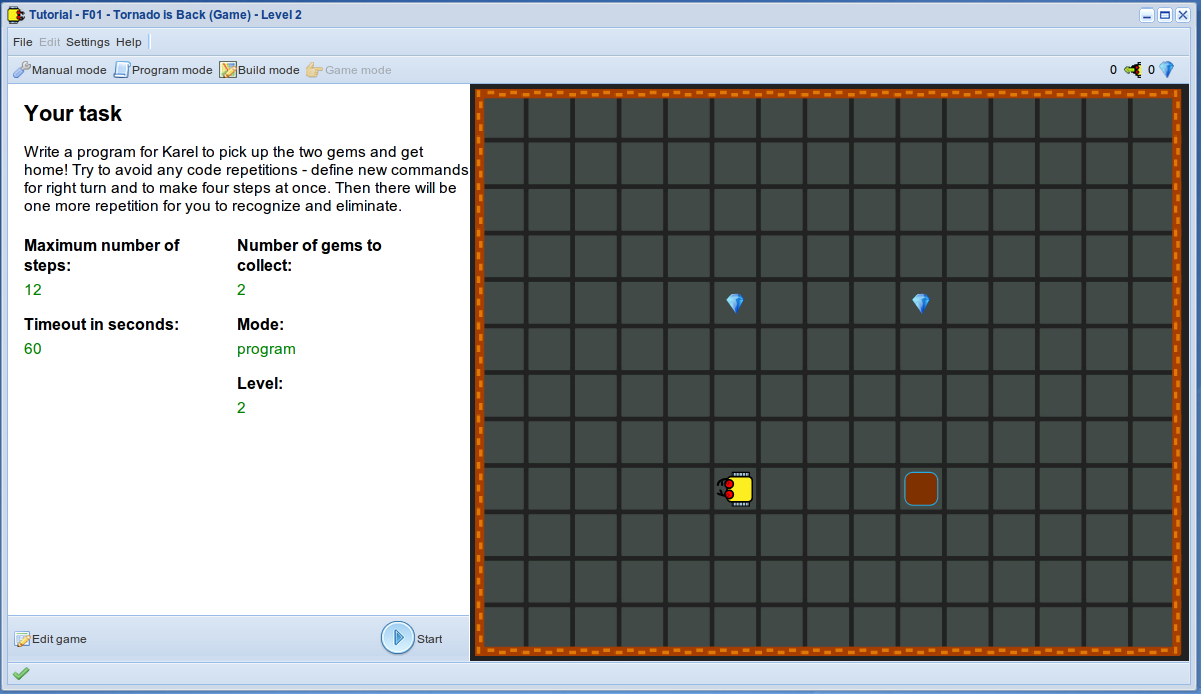
\includegraphics[width=0.7\textwidth]{img/f01.png}
\end{center}
\vspace{-4mm}
\caption{Karel needs to collect four stars of gems.}
\label{fig:f01}
\vspace{-10mm}
\end{figure}
\noindent

\subsection{F02 - U-Haul}

{\em Write a program for the robot to move the 6x6 square of gems to the opposite corner of the maze. The task is finished when the robot is back home.}


\begin{figure}[!ht]
\begin{center}
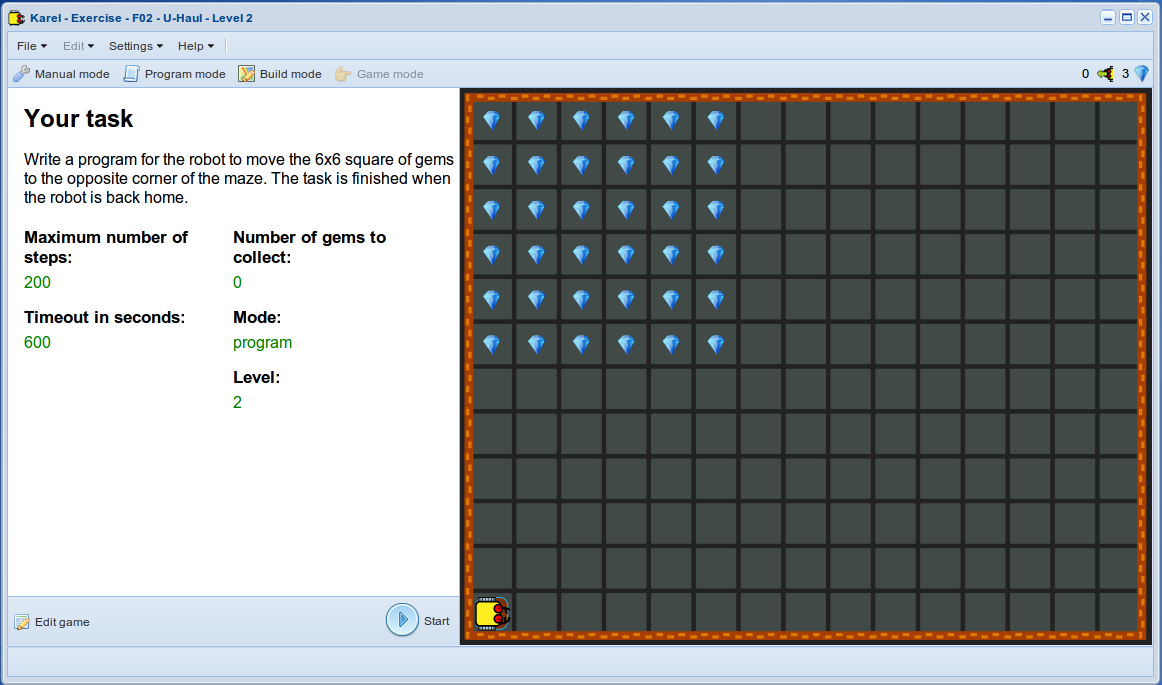
\includegraphics[width=0.7\textwidth]{img/f02.png}
\end{center}
\vspace{-4mm}
\caption{Karel needs to move the gems to the opposite corner of the maze.}
\label{fig:f02}
\vspace{-10mm}
\end{figure}
\noindent

\subsection{F03 - Egg Hunt}

{\em Write a program for Karel to search all cells and collect all eggs (gems) that he can find. The task is finished when the robot is back home.}


\begin{figure}[!ht]
\begin{center}
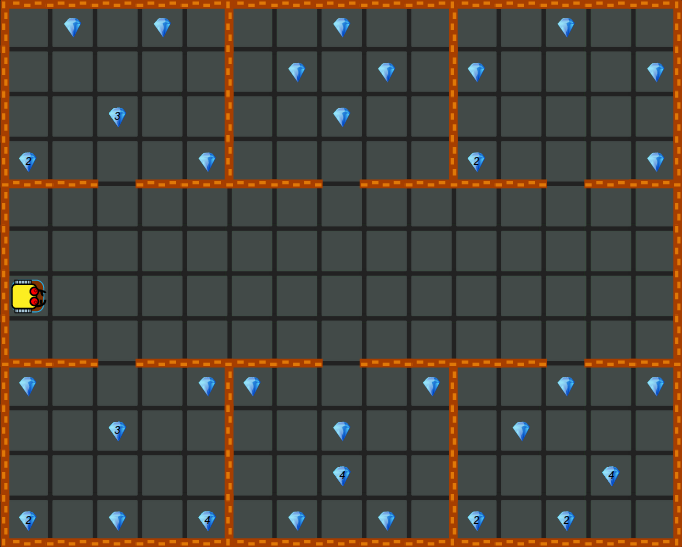
\includegraphics[width=0.7\textwidth]{img/f03.png}
\end{center}
\vspace{-4mm}
\caption{Easter is here, Karel is on egg hunt!}
\label{fig:f03}
\vspace{-10mm}
\end{figure}
\noindent

\subsection{F04 - Blind Carpenter}

{\em Karel is a blind carpenter who needs to install windows (gems) into a newly built house. All he knows is that the house is a rectangle and that each window is exactly one tile large, But he can't see where the openings for the windows are. Install the windows and return home!}


\begin{figure}[!ht]
\begin{center}
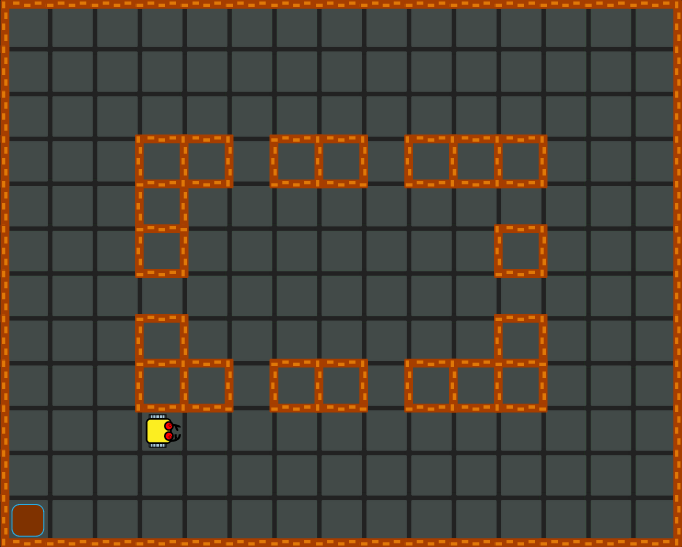
\includegraphics[width=0.7\textwidth]{img/f04.png}
\end{center}
\vspace{-4mm}
\caption{This time Karel installs windows.}
\label{fig:f04}
\vspace{-10mm}
\end{figure}
\noindent



\subsection{F05 - Pirate Ship}

{\em Karel is on a pirate ship! Write a program for him to collect all 
gems and run away (to his home) before the pirates are back. Here Karel 
needs to be extremely efficient to survive. Therefore, there should be 
no repeating parts whatsoever in your program!}


\begin{figure}[!ht]
\begin{center}
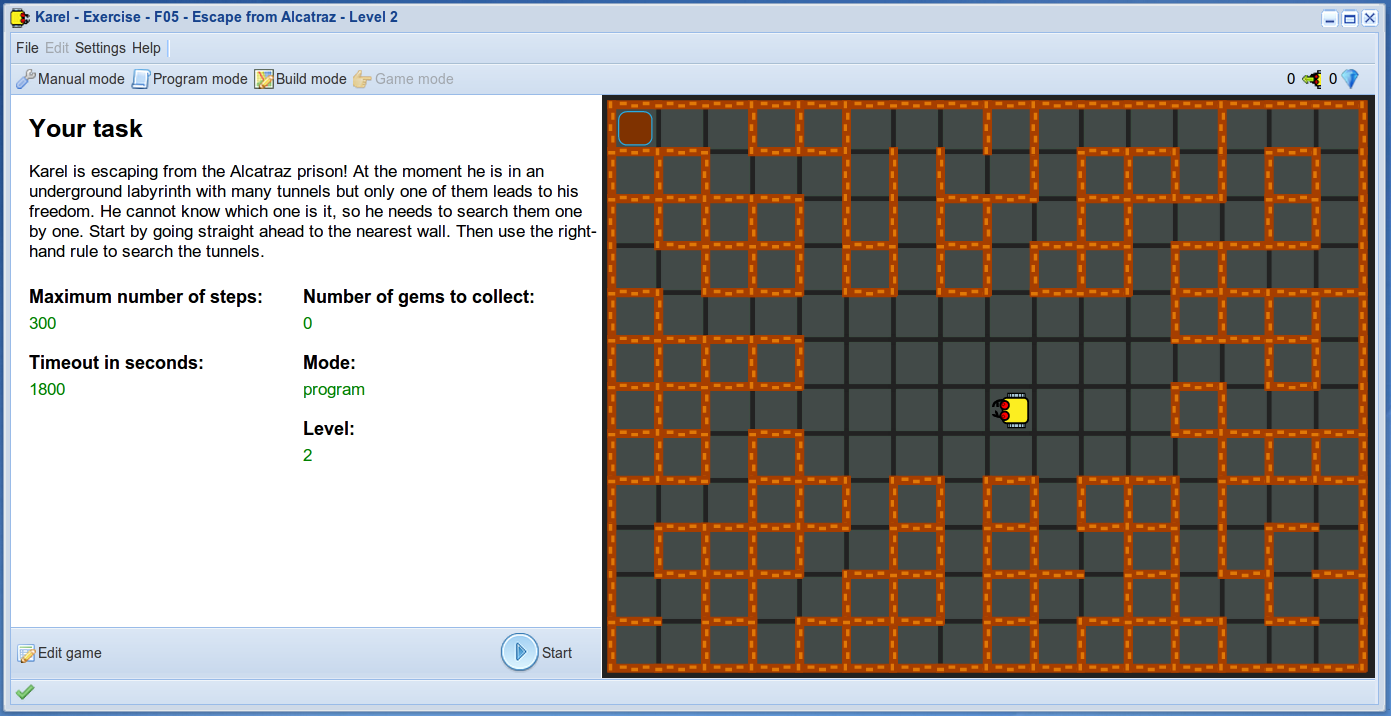
\includegraphics[width=0.7\textwidth]{img/f05.png}
\end{center}
\vspace{-4mm}
\caption{Karel found a pirate treasure.}
\label{fig:f05}
\vspace{-10mm}
\end{figure}
\noindent


\subsection{F06 - Diamond Staircase}

{\em Write a program for Karel to climb the stairs, collect all gems, and get home!}
\newpage

\begin{figure}[!ht]
\begin{center}
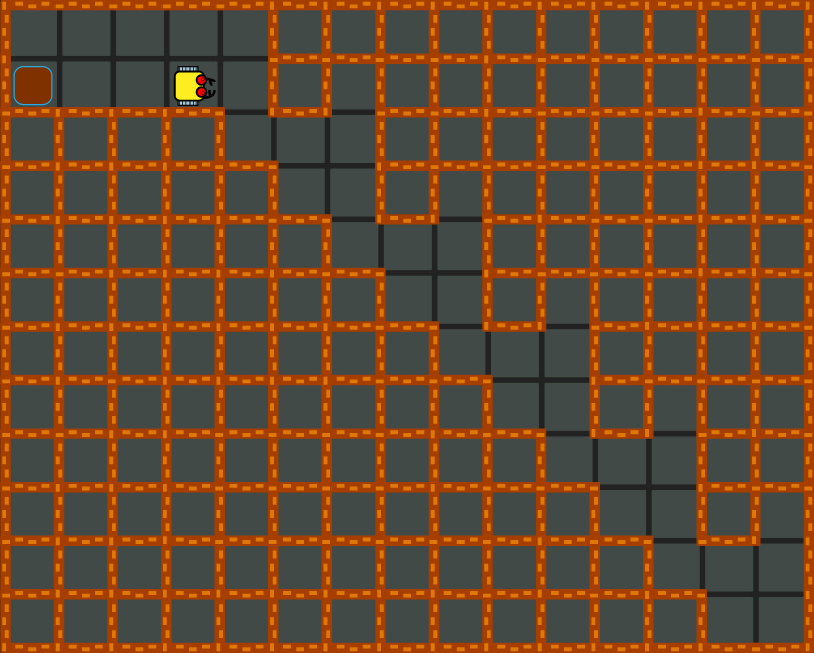
\includegraphics[width=0.7\textwidth]{img/g01.png}
\end{center}
\vspace{-4mm}
\caption{This time Karel has to do some climbing.}
\label{fig:g01}
\vspace{-4mm}
\end{figure}
\noindent


\subsection{F07 - Plucking Flowers}

{\em Write a program for Karel to pluck all flowers that grow at the fence of his garden (gems), and get back home! Note two level of repetitions - the fence has four edges, and it takes 7 steps to walk each edge.}


\begin{figure}[!ht]
\begin{center}
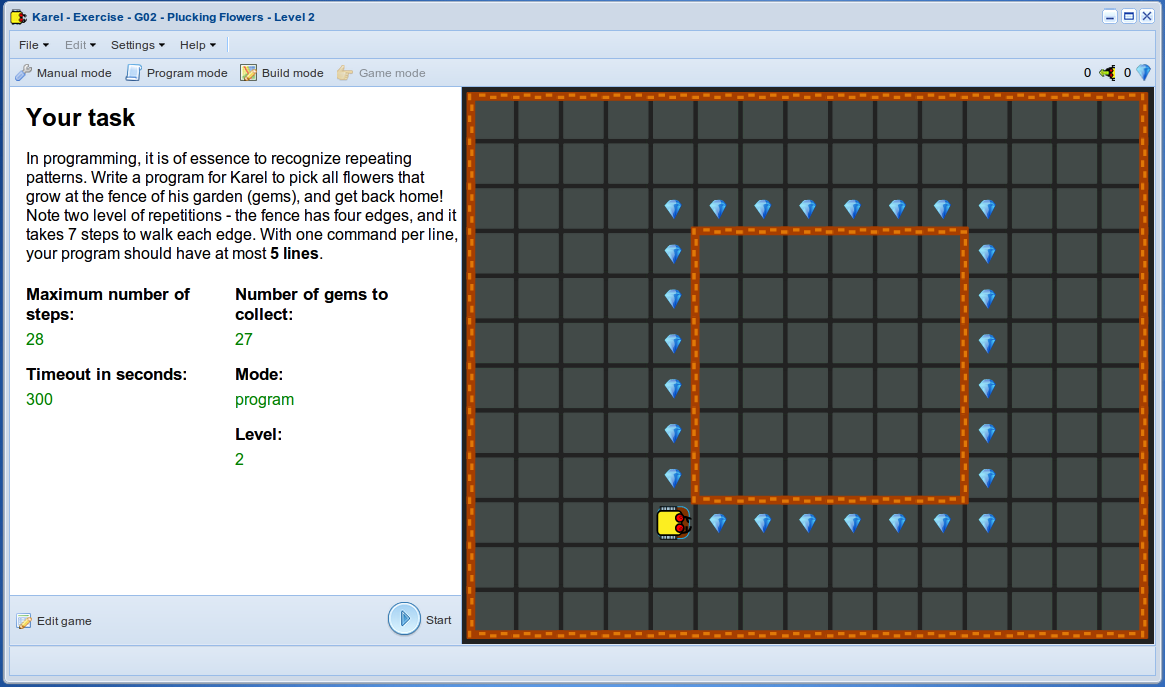
\includegraphics[width=0.7\textwidth]{img/g02.png}
\end{center}
\vspace{-4mm}
\caption{Karel is plucking flowers along his fence.}
\label{fig:g02}
\vspace{-4mm}
\end{figure}
\noindent

\subsection{F08 - Gems for Friends}

{\em Karel has three gems in his bag, that he wants to give to his three friends R2, D2 and Marvin who live close by. They are very good friends, so Karel is allowed to enter their homes at any time. Write a program for Karel to put a gem on the ground in the middle of each friend's home, and then get back to his own house! Hint: There will be an outer loop of four repetitions, that will contains inner repetitions in it.}


\begin{figure}[!ht]
\begin{center}
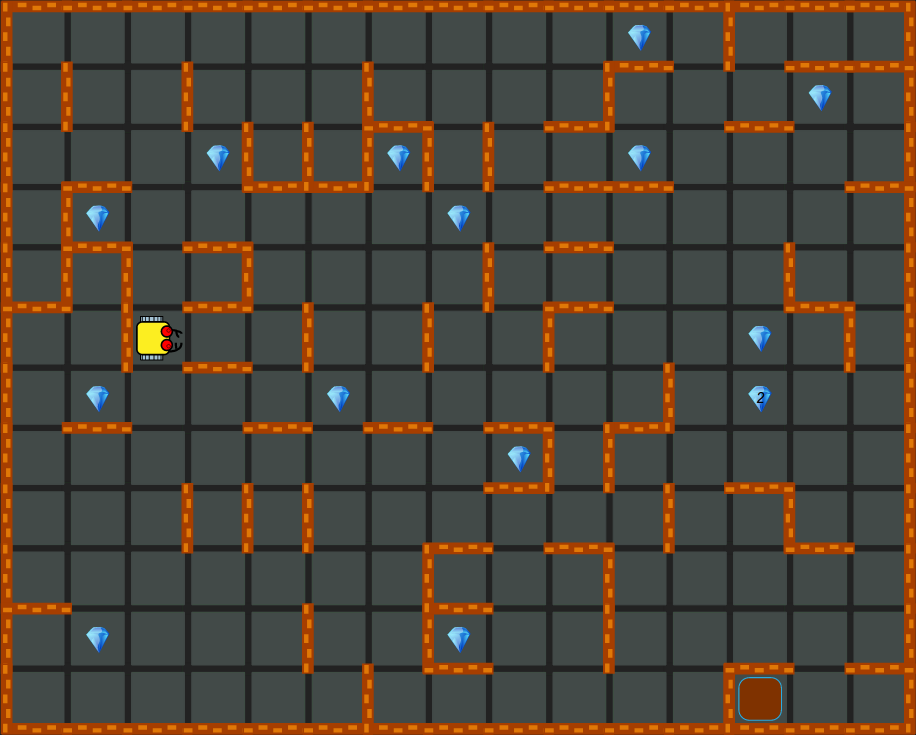
\includegraphics[width=0.7\textwidth]{img/g03.png}
\end{center}
\vspace{-4mm}
\caption{Karel is going to give gems to his three friends R2, D2 and Marvin.}
\label{fig:g03}
\vspace{-4mm}
\end{figure}
\noindent

\subsection{F09 - Diamond Rectangle}

{\em Karel stands in front of a rectangle with unknown dimensions. He knows that the rectangle is surrounded with gems. Sometimes the gems are piled up, but he does not know how many gems are in each pile. Write a program for the robot to walk around the rectangle, collect all gems, and get home!}

\newpage

\begin{figure}[!ht]
\begin{center}
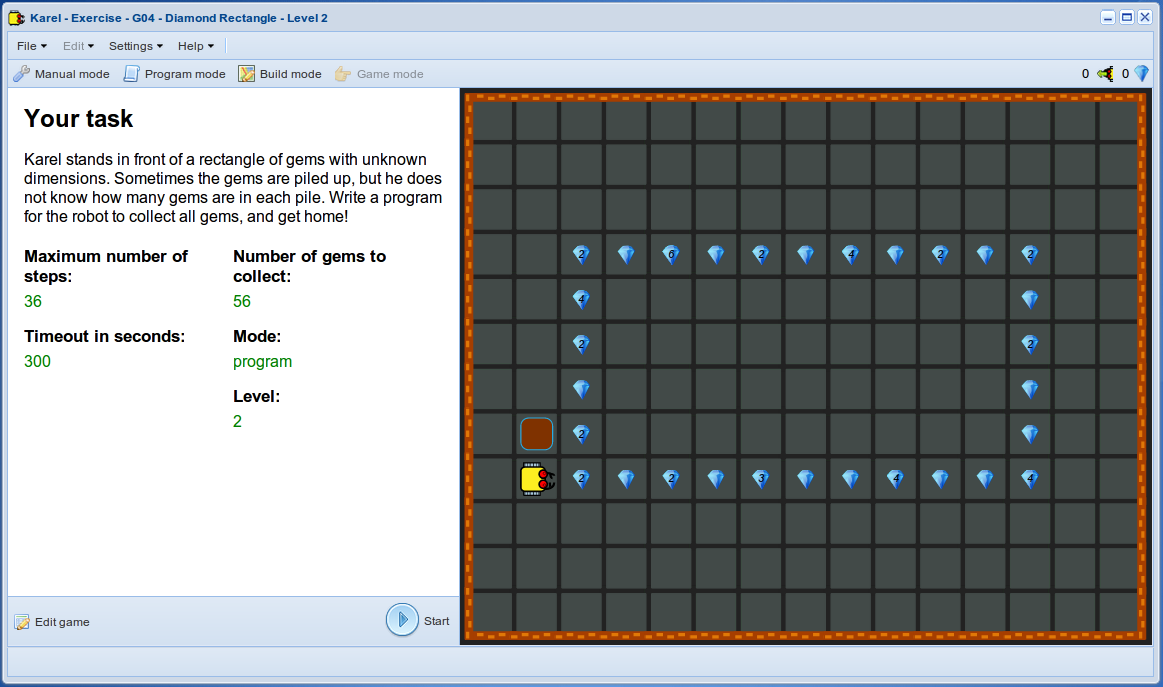
\includegraphics[width=0.7\textwidth]{img/g04.png}
\end{center}
\vspace{-4mm}
\caption{This time Karel does not know the size of the rectangle.}
\label{fig:g04}
\vspace{-10mm}
\end{figure}
\noindent

\subsection{F10 - Gem Jam!}

{\em In this maze, gems are distributed randomly along the walls. Otherwise 
the maze is empty. Karel's home is in the south-west corner, and the robot 
stands on the right of it, facing east. Write a program for Karel to collect 
all the gems and return home!}

\begin{figure}[!ht]
\begin{center}
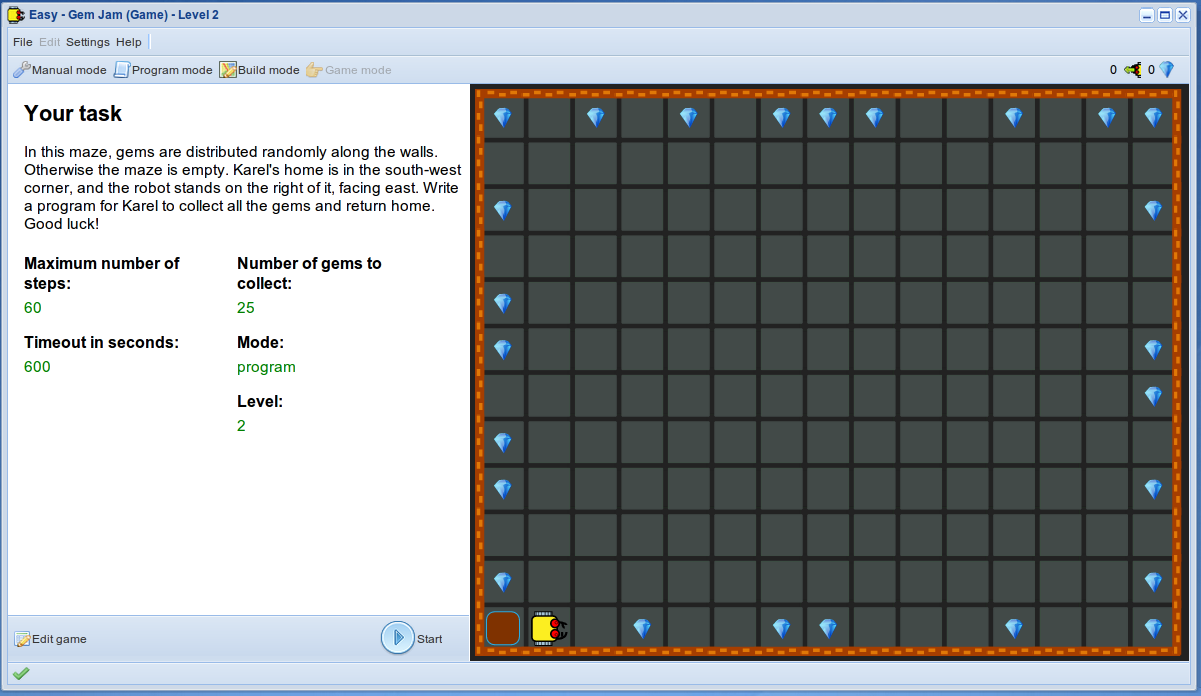
\includegraphics[width=0.7\textwidth]{img/g05.png}
\end{center}
\vspace{-4mm}
\caption{Gem Jam!}
\label{fig:g05}
\vspace{-10mm}
\end{figure}
\noindent

\newpage

\subsection{F11 - The Matrix}

{\em Write a program for Karel to collect all gems and get back home! The record is 
210 steps made. Can you do it with fewer steps?}

\begin{figure}[!ht]
\begin{center}
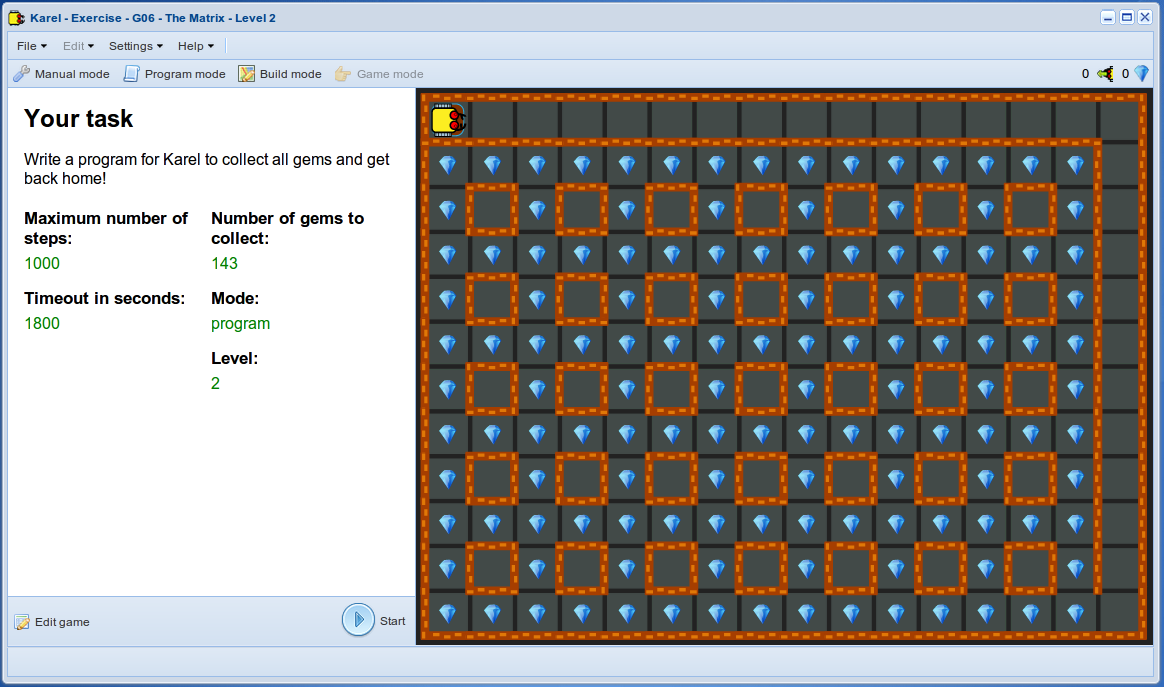
\includegraphics[width=0.7\textwidth]{img/g06.png}
\end{center}
\vspace{-4mm}
\caption{The Matrix.}
\label{fig:g06}
\vspace{-10mm}
\end{figure}
\noindent

\subsection{F12 - Escape from Alcatraz}

{\em Karel is escaping from the Alcatraz prison! At the moment he is in an underground labyrinth with many tunnels but only one of them leads to his freedom. He cannot know which one is it, so he needs to search them one by one. Start by going straight ahead to the nearest wall. Then use the right-hand rule to search the tunnels.}

\newpage

\begin{figure}[!ht]
\begin{center}
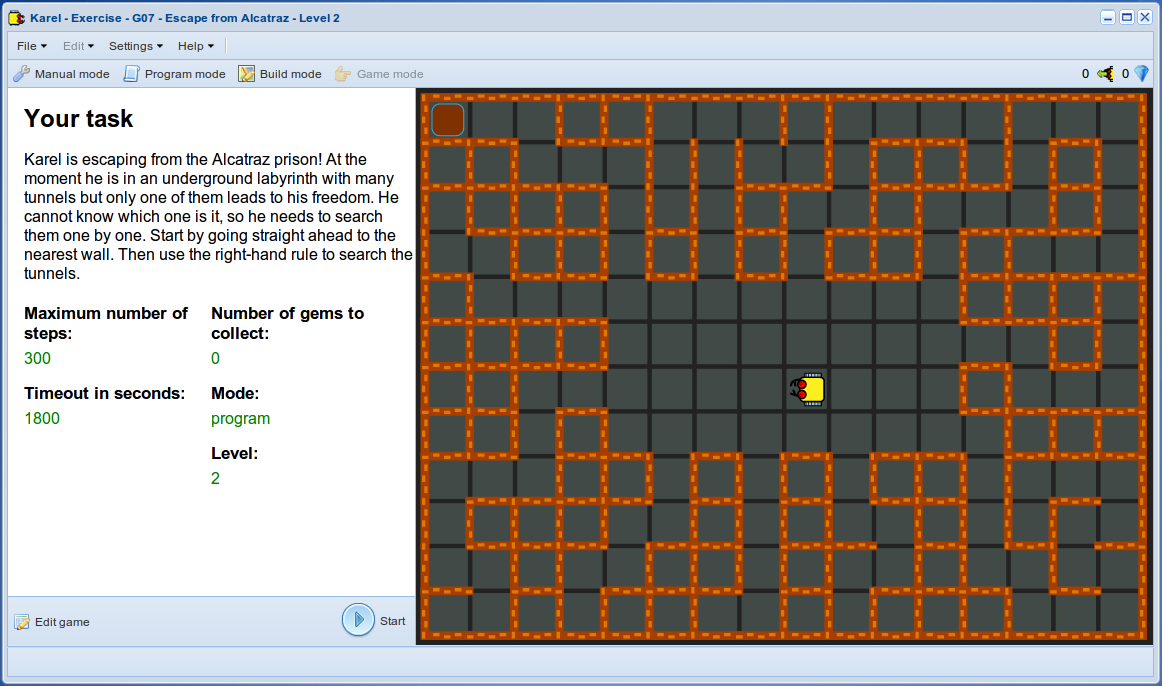
\includegraphics[width=0.7\textwidth]{img/g07.png}
\end{center}
\vspace{-4mm}
\caption{Karel is escaping from the Alcatraz prison.}
\label{fig:g07}
\vspace{-8mm}
\end{figure}
\noindent

\subsection{F13 - Border Patrol}

{\em Write a program for Karel to check the perimeter of the maze using the 
right-hand rule. Do not forget to pick up all gems that you find on the way.}

\begin{figure}[!ht]
\begin{center}
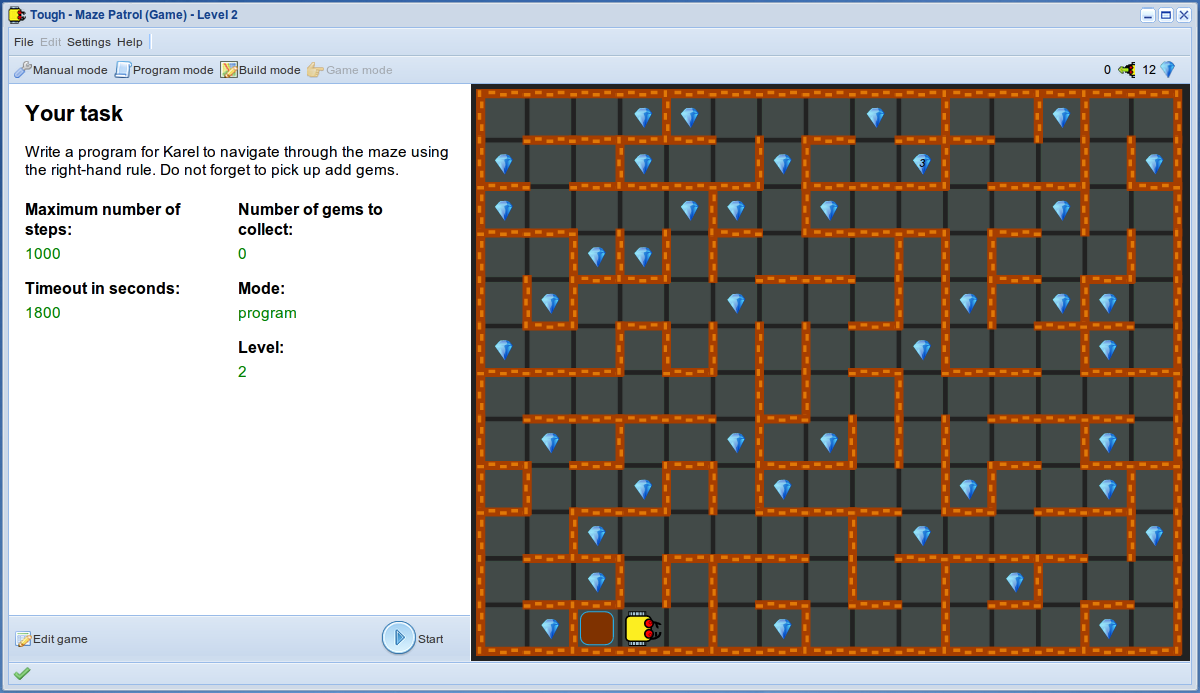
\includegraphics[width=0.7\textwidth]{img/g08.png}
\end{center}
\vspace{-4mm}
\caption{Border Patrol.}
\label{fig:g08}
\vspace{-10mm}
\end{figure}
\noindent

\subsection{F14 - Ariadne's Thread}

{\em In an ancient Greek legend, princess Ariadne saved the life of her 
beloved Theseus by giving him a thread that he used to avoid getting lost 
in the maze of king Minos and kill a feared beast Minotaurus. Karel uses 
a similar technique - he leaves behind him a chain of gems that helps him 
to safely find his way back home. Your program needs to work for an 
arbitrary maze. You can assume that the string of gems is continuous 
and that it does not contain any loops.}

\begin{figure}[!ht]
\begin{center}
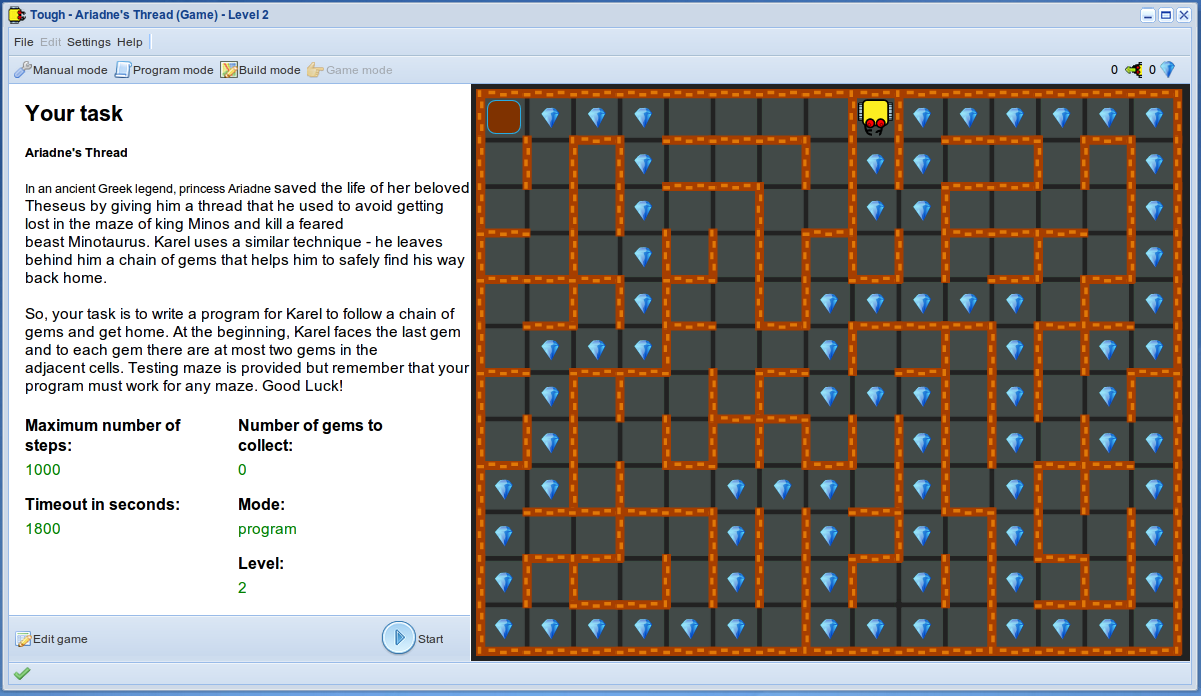
\includegraphics[width=0.7\textwidth]{img/g09.png}
\end{center}
\vspace{-4mm}
\caption{Maze of king Minos, home of the beast Minotaurus.}
\label{fig:g09}
\vspace{-10mm}
\end{figure}
\noindent

\section{Part G - Using Variables}

As usual, all games in this section can be cloned via the File Manager's
Project menu. 

\subsection{G01 - Numerology I}

{\em Each box contains an integer number between 0 and 9. The numbers are not known to Karel a-priori. He needs to enter each box and recognize the number in it. Let's call this number N. When he leaves the box, he needs to create a pile of N gems. The task finishes when this is done for all boxes and the robot gets home.}

\newpage

\begin{figure}[!ht]
\begin{center}
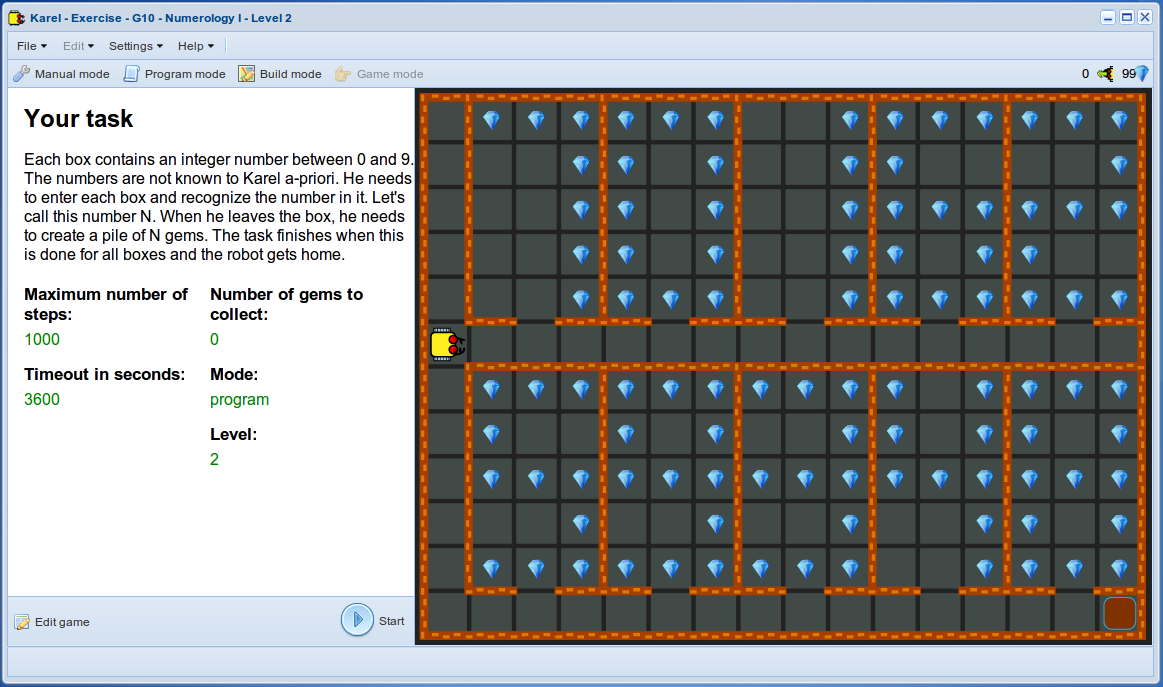
\includegraphics[width=0.7\textwidth]{img/g10.png}
\end{center}
\vspace{-4mm}
\caption{Karel decided to become a numerologist.}
\label{fig:g10}
\vspace{-4mm}
\end{figure}
\noindent

\subsection{G02 - Numerology II}

{\em There is a pile of N gems before the entrance to the box. It is known that N is between zero and 9. Karel needs to enter the box and render the number N. The task finishes when this is done and the robot gets home.}


\begin{figure}[!ht]
\begin{center}
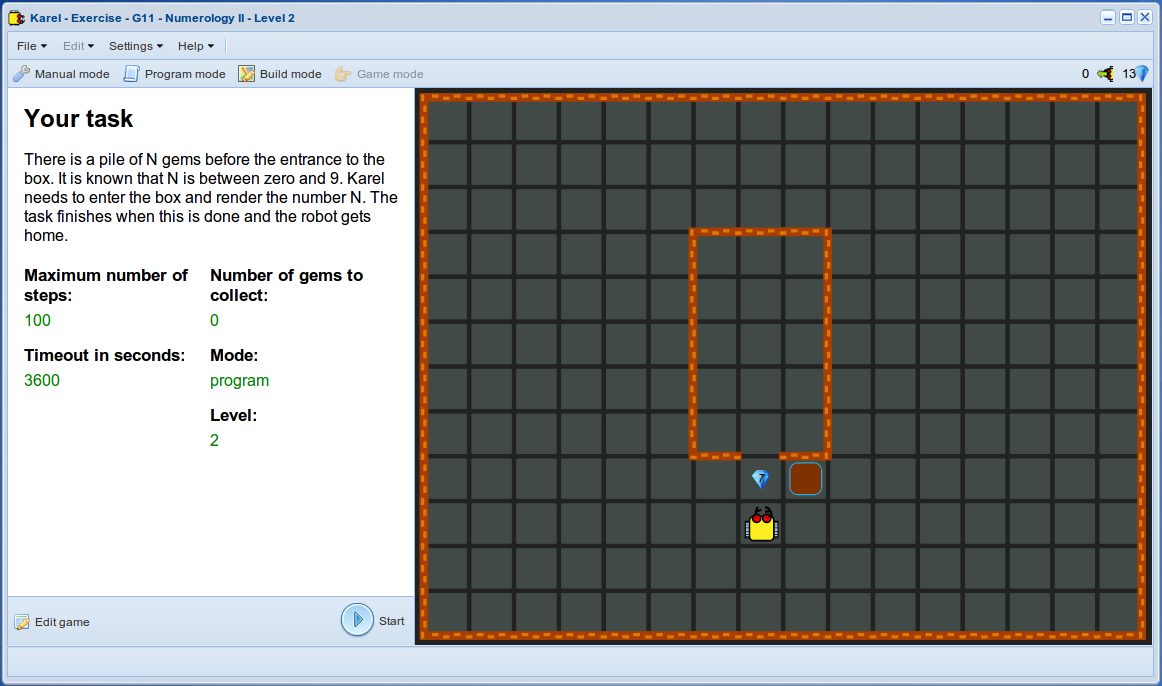
\includegraphics[width=0.7\textwidth]{img/g11.png}
\end{center}
\vspace{-4mm}
\caption{Karel is typing numbers.}
\label{fig:g11}
\vspace{-4mm}
\end{figure}
\noindent

\subsection{G03 - Numerology III}

{\em Add the numbers! Remember - Karel cannot see what numbers are in the boxes as you can see them. They can be any integers between 0 and 9. The task finishes when the robot gets home.}


\begin{figure}[!ht]
\begin{center}
\includegraphics[width=0.7\textwidth]{img/g12.png}
\end{center}
\vspace{-4mm}
\caption{Adding numbers without using math!}
\label{fig:g12}
\vspace{-4mm}
\end{figure}
\noindent

\subsection{G04 - Eight Queens}

{\em Karel stands on an 8 x 8 chess board along with eight queens (the gems). Recall that a chess queen dominates its row, its column, as well as both diagonals that pass through her position. Nothing may stand in these fields or she will destroy it. Currently, some queens are threatening each other. Write a program for Karel to correct the positions of the queens in such a way that none of them is threatened. Your program should be able to do it for any initial distribution of the queens. Enter the home after you are finished.}

\newpage

\begin{figure}[!ht]
\begin{center}
\includegraphics[width=0.7\textwidth]{img/g14.png}
\end{center}
\vspace{-4mm}
\caption{The famous eight queens problem.}
\label{fig:g14}
\vspace{-4mm}
\end{figure}
\noindent

\subsection{G05 - BubbleSort}

{\em Karel stands in front of four piles of gems, let's enumerate them by 1, 2, 3 and 4. He does not know how many gems are in each pile. All he knows is that each pile contains between 1 and 4 gems, and that two or more piles can be equally large. Sort the piles in such a way that the smallest pile is on the left and the largest on the right. Use the BubbleSort algorithm: Implement a function that switches two adjacent piles if the one on the right has fewer gems than the one on the left. Apply this function to piles 1 and 2, then to piles 2 and 3, then to piles 3 and 4. Now it is certain that the largest number is on the right-most position! Next, do the same for just the first three piles. Last, apply the function to piles 1 and 2, and you are done! }

\newpage 

\begin{figure}[!ht]
\begin{center}
\includegraphics[width=0.7\textwidth]{img/g13.png}
\end{center}
\vspace{-4mm}
\caption{Karel is sorting four piles of gems.}
\label{fig:g13}
\vspace{-4mm}
\end{figure}
\noindent








\section{What Next?}

Congratulations on making it to the end of the tutorial! We hope that you
enjoyed it. If you can think of any ways to improve the application 
Karel the Robot in NCLab or this tutorial, please let us know. If you 
feel capable of solving the last two problems, make sure to send us your 
solution. We are also thinking of creating a Gallery of Games just for Karel,
so if you have a nice game, please let us know as well. 

Although you may feel like an Almighty Programmer right now, we would
recommend staying humble. Even the most experienced programmers are
learning new things all the time. If you enjoy programming, your next 
language to learn may be Python. We have a Python Programming tutorial
in NCLab for you. We would also recommend that you learn Javascript since this 
is the most popular language for web development. Depending on your 
other hobbies or interests, C++ or even Fortran might be interesting. 
In any case, the NCLab Team wishes you good luck, and keep us in your 
favorite bookmarks!\\
\\
\hbox{} \hfill Your NCLab Team






\end{document}
